\documentclass[11pt, a4paper, spanish]{article}

%%%%%%%%%% COMIENZO DEL PREAMBULO %%%%%%%%%%

%Info sobre este documento
\author{Martin Cammi}
\title{Trabajo Pr'actico de Ingenier'ia del software I}

%\usepackage{infostyle}                                                  % provee un look & feel similar a un documento Word
\usepackage[top=2.5cm, bottom=2.5cm, left=2.5cm, right=2.5cm]{geometry}  % m\'argenes
\usepackage[ansinew]{inputenc}                                           % permite que los acentos del estilo \'a\'e\'i\'o\'u salgan joya
\usepackage[spanish, activeacute]{babel}                                 % idioma espa\~{n}ol, acentos f\'aciles y deletreo de palabras
\usepackage{indentfirst}                                                 % permite indentar un parrafo a mano
\usepackage{caratula}                                                    % incluye caratula est\'andar
\usepackage{graphicx}                                                    % permite insertar gr\'aficos
\usepackage{color}                                                       % permite el uso de colores en el documento
\usepackage[pdfcreator={TexLive!, LaTeX2e con TeXnicCenter y la inteligencia de Jonathan ;-)},
			pdfauthor={Grupo 1"},
			pdftitle={Ingenieria del Software - Trabajo practico: sistema de software CentralMarket},
			pdfsubject={Trabajo Practico de Modelado de dominio},
			pdfkeywords={Contenidos, proveedor, bajo demanda},
			pdfstartview=FitH,            % Fits the width of the page to the window
			bookmarksnumbered,            % los bookmarks numerados se ven mejor...
			colorlinks,                   % links con bellos colores
			linkcolor=magenta]            % permite cambiar el color de los links
			{hyperref}                    % Permite jugar con algunas cosas que aparecer\'an en el PDF final
\usepackage{hyperref}


%\selectlanguage{spanish}

\linespread{1.3}                    % interlineado equivalente al 1.5 l\'ineas de Word...
\pagestyle{myheadings}              %encabezado personalizable con \markboth{}{}
\markboth{}{Trabajo Modelado de Objetivos. (Abreg\'u, Cammi, De Sousa, M\'endez, Raffo) }
\headsep = 30pt                     % separaci\'on entre encabezado y comienzo del p\'arrafo

%\addtolength{\oddsidemargin}{-2cm}	% configuracion IDEAL!!!
%\addtolength{\textwidth}{4cm}
%\addtolength{\textheight}{2cm}

% macro 'todo' para To-Do's
\def\todo#1{\textcolor{red}{#1}}

% Macro 'borde' para un texto con borde
\newsavebox{\fmbox}
\newenvironment{borde}[1]
{\begin{lrbox}{\fmbox}\begin{minipage}{#1}}
{\end{minipage}\end{lrbox}\fbox{\usebox{\fmbox}}\\[10pt]}

%%%%%%%%%% FIN DEL PREAMBULO %%%%%%%%%%

\begin{document}

\materia{Ingenier\'ia de Software I}
\submateria{Primer Cuatrimestre de 2012}
\titulo{Trabajo pr\'actico 2}
\subtitulo{Modelos de comportamiento del sistema de software para CentralMarket}
\grupo{Grupo 1}

\integrante{Abreg\'u, Angel}{082/09}{angelj\_a@hotmail.com}
\integrante{Cammi, Mart\'in}{676/02}{martincammi@gmail.com}
\integrante{De Sousa, Mariano}{389/08}{marian\_sabianaa@hotmail.com}
\integrante{M\'endez, Gonz\'alo}{843/04}{gemm83@hotmail.com}
\integrante{Raffo, Diego}{423/08}{enanodr@hotmail.com}


\maketitle

\thispagestyle{empty}

\tableofcontents

\newpage

% Conviene poner las secciones como diferentes archivos,
% sobre todo cuando se trabaja en equipo.
% Es m\'as f\'acil para sincronizar mediante control de versiones.
%\input{Introducci\'on}


% BEGIN Ejemplos de uso

	%\section{Una secci\'on}
	%\label{sec:unaSeccion}
	%Hola! Soy una Secci\'on
	%	\subsection{Una subsecci\'on}
	%		Y yo soy una subsecci\'on!!!
	%		\subsubsection{Una subsubsecci\'on}
	%			Y yo soy una sub-subsecci\'on!!!
	%			\paragraph{Un p\'arrafo\\}
	%				Y yo soy un p\'arrafo, porque no hay mas sub-sub-sub-subsecciones!!!

	%\section{Otra secci\'on}
	%	Como pudimos ver en la secci\'on \ref{sec:unaSeccion}, esto es una demo de una referencia a una secci\'on.
	
	%	Tambi\'en podemos hacer referencia a la p\'agina de la secci\'on:\\[10pt]
	
		% Ejemplo de uso de un borde (falta pulir para que no tire un warning!)
	%	\begin{borde}{0.98\textwidth}
	%		En la p\'agina \pageref{sec:unaSeccion}, hay una secci\'on pilla...
	%	\end{borde}

% END Ejemplos de uso


\section{Propuesta de servicios}
\label{sec:Propuesta de servicios}

\subsection{Introducci\'on}

	Tras haber realizado una serie de iteraciones con los directivos de CentralMarket sobre la \'ultima presentaci\'on del sistema y en base
a las correciones y ajustes que nos han comentado quieren, hemos armado una nueva serie de documentos para detallar mejor el comportamiento del sistema.
A tal efecto hemos revisado una serie de puntos con los directivos y se han modificado algunos:


\begin{itemize}
	
	\item{ Los agentes \emph{Gerente de proyecto} y \emph{Desarrollador} que figuraban en el diagrama de objetivos de la documentaci\'on revisada con el cliente no 			ser\'an tenidos en cuenta en esta etapa ya que forman parte intr\'inseca de la construcci\'on del mismo y no de su comportamiento.}

	\item{ El agente \emph{Cliente} ser\'a modelado en esta etapa a trav\'es del usuario quien es el que interact\'ua directamente con el sistema)}

	\item{ De las diferentes opciones propuestas para el tipo de descarga (no streaming) los directivos han optado por la descarga directa.}
	
	\item{ Del diagrama de objetivos, la rama 3.1 (Soportar TV, PC, tablet y mobile) no ser\'a modelada en esta etapa ya que un equipo especial de CentralMarket
se ocupar\'a de definir esas necesidades.}

	\item{ Del mismo modo la Situaci\'on 6 mencionada en la documentaci\'on anterior sobre la \emph{Actualizaci\'on de la interfaz de usuario} no ser\'a incluida en esta nueva presentaci\'on ya que CentralMaket se ocupar\'a tambi\'en }

	\item{ En el modelado a continuaci\'on asumiremos que todos los actores que interactuen con el sistema ya tienen creada una cuenta previa para poder loguearse y realizar sus acciones }

	\item{ Consultamos a la analista de CentralMarket al respecto de los tipos de publicidad y tipos de posicionamiento y nos coment\'o que dej\'eramos la definici\'on de estos tipos a ellos con lo cual asumiremos que ya est\'an definidos en el sistema}

	\item{ La analista tambi\'en hizo incapi\'e en que es importante que el Administrador de contenidos tenga una forma de "poner online" los contenidos que 
ya han sido verificados, es por eso que le hemos otorgado la opci\'on de "Habilitar" los contenidos cuando quiere ponerlos online}

	\item{ Los directivos nos nos mencionaron que quieren poder ver claramente cual es el flujo de validaci\'on de los contenidos, para asegurarse de brindar
la mejor calidad aunque para los contenidos en si quieren poder asegurar no llegar a generar inconsistencias en el sistema. Es por eso que decidimos presentarles
todo lo referente a revisi\'on de contenidos en un \emph{Casos de Uso} y un \emph{Diagramas de actividad} y con relaci\'on a los contenidos en si agregar tambi\'en un \emph{Modelo Conceptual}}

	\item{ Al consultar sobre los paquetes los directivos nos comentaron que en una primera instancia no implementar\'an paquetes, quiz\'as m\'as adelante, as\'i que no quieren demasiada informaci\'on sobre ellos, decidimos no agregarlos en el \emph{Modelo conceptual} para simplificar la descripci\'on de los contenidos ya que en un 
futuro puede extenderse.}



\end{itemize}

	
\section{Diagramas}
	
	A continuaci\'on presentamos una serie de modelos que representan el comportamiento acordado con los directivos de CentralMarket.
Presentaremos las funcionalidades con tres tipos de diagramas: de \emph{Casos de Uso}, de \emph{Actividad} y \emph{Modelo Conceptual}.\\

	Un diagrama de \emph{Casos de Uso} permite identificar claramente la interacci\'on del sistema con diferentes actores. A continuaci\'on se muestran todos los actores relevantes al sistema y las acciones que pueden realizar con el sistema.

\newpage

\subsection{Diagrama de Casos De Uso}


	\begin{center}
		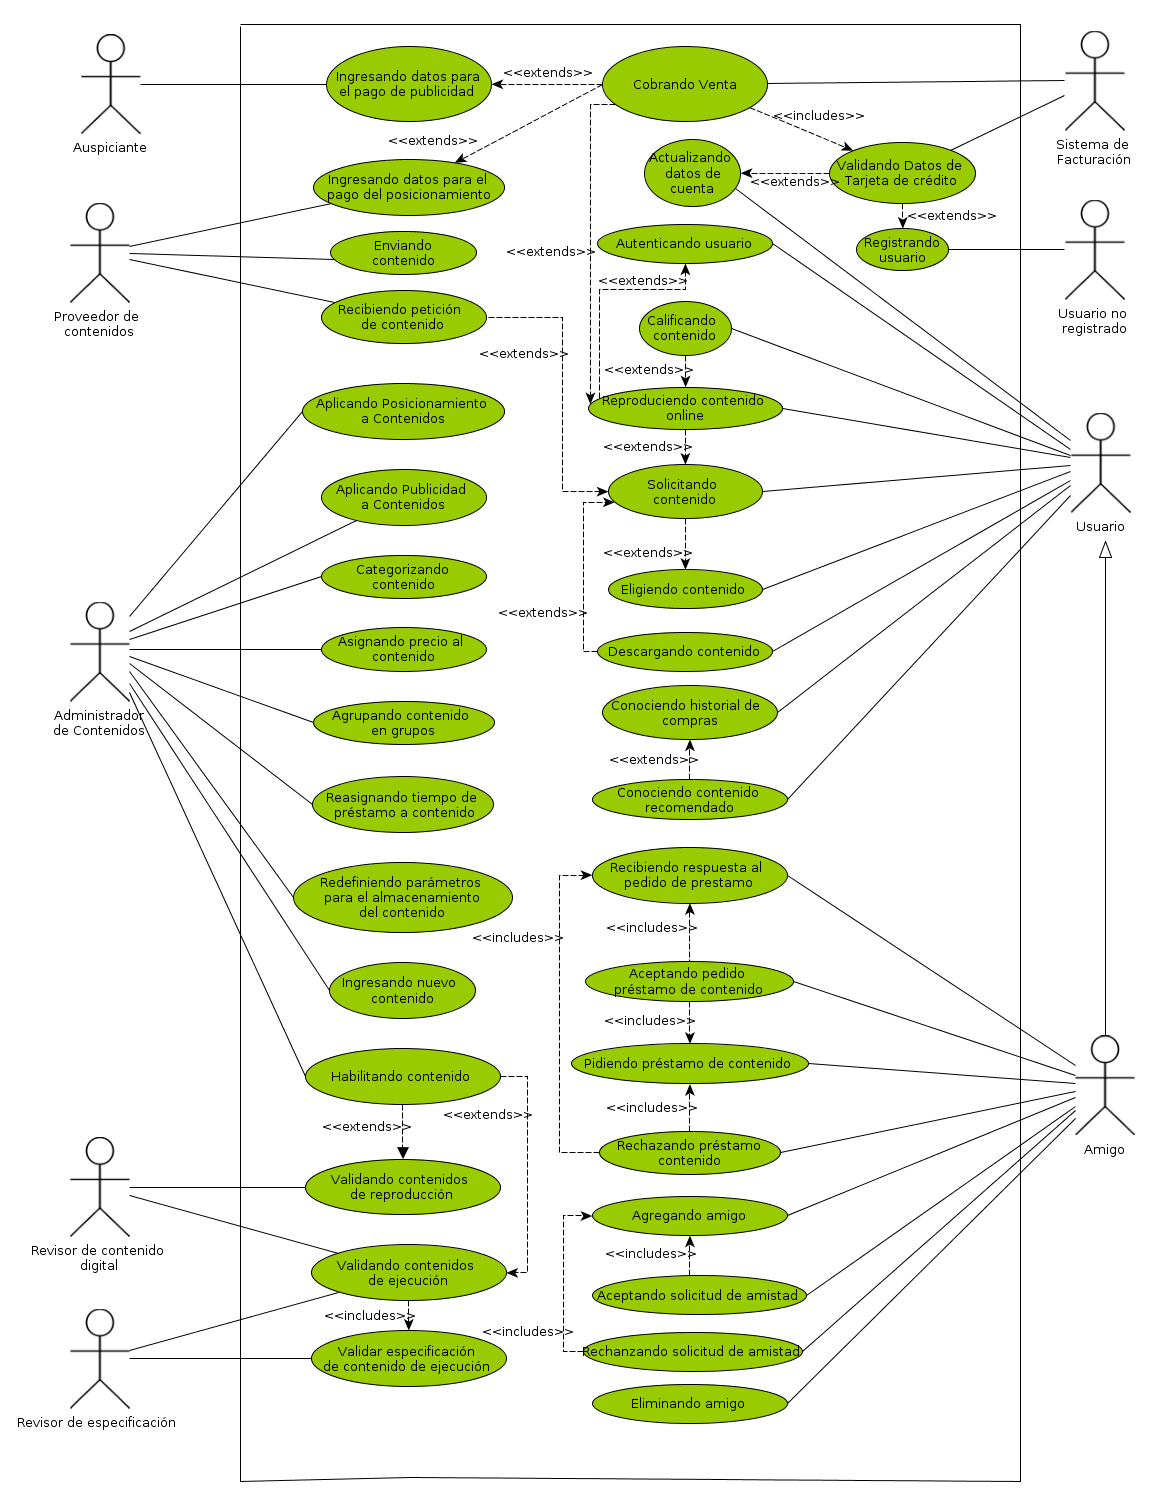
\includegraphics[scale=0.37]{Diagramas/01-CasosdeUsoCU.png}
	\end{center}

\newpage

\subsection{Descripci\'on de los casos de uso.}

\begin{center} \line(1,0){450} \end{center}
\noindent{\textbf{Caso de uso: Eligiendo contenido.}} \\
\textbf{Actores:} Usuario. \\
\textbf{Pre:} El usuario est\'a registrado y autenticado. \\
\textbf{Post:} El usuario eligi\'o un contenido.\\

\noindent{\textbf{\underline{Caso normal}}}

\begin{enumerate}
	\item El usuario entra a la b\'usqueda de contenido en el sistema.
	\item El usuario ingresa un t\'ermino en la b\'usqueda de acuerdo al contenido que quiera buscar y/o marca los filtros que necesite.
	\item El sistema ofrece una lista b\'asica de contenidos acorde al usuario y los filtros completados.
	\item El usuario ve que el contenido a buscar forma forma parte de lista seleccionada y accede a al detalle.
	\item El usuario decide si va a consumir el contenido, de ser as\'i, extiende caso de uso "Solicitando contenido"
	\item \textbf{Fin Caso de uso}
\end{enumerate}

\noindent{\textbf{\underline{Caso alternativo}}} \\

4.1 - El usuario no encuentra el contenido que est\'a buscando y decide
hacer una b\'usqueda diferente, va al paso 2.

\begin{center} \line(1,0){450} \end{center}

\newpage

\begin{center} \line(1,0){450} \end{center}

\noindent{\textbf{Caso de uso: Solicitando contenido. }} \\
\textbf{Actores:} Usuario. \\
\textbf{Pre:} El usuario est\'a autenticado y ha elegido un contenido. \\
\textbf{Post:} El usuario solicit\'o un contenido.\\

\noindent{\textbf{\underline{Caso normal}}} 

\begin{enumerate}
	\item El sistema muestra al usuario, dado el tipo de contenido, cu\'ales son las modalidades para consumirlo (descarga y/o streaming)
	\item El usuario selecciona la modalidad que va utilizar.
	\item El sistema valida que el dispositivo est\'e soportado para iniciar el proceso de descarga o streaming.
	\item Si la cuenta no tiene asociada una tarjeta, el sistema pide una, el usuario ingresa los datos.
	\item Extiende Caso de Uso "Cobrando venta"
	\item Si es descarga, extiende Caso de Uso "Descargando contenido"; si el contenido es soportado y es streaming extiende Caso de Uso "Reproduciendo contenido online"
	\item \textbf{Fin Caso de uso}
\end{enumerate}

\noindent{\textbf{\underline{Caso alternativo}}} \\

\noindent{3.1 - El sistema muestra mensaje de error indicando que el dispositivo no est\'a soportado. Ir a 7.}\\
4.1 - Si el contenido es gratuito, ir a 6.\\
6.1 - De no ser v\'alida la tarjeta, el sistema muestra mensaje de error y vuelve a 4.\\
6.2 - De no ser exitoso el cobro, el sistema muestra mensaje de error.\\

\begin{center} \line(1,0){450} \end{center}

\newpage 

\begin{center} \line(1,0){450} \end{center}

\noindent{\textbf{Caso de uso: Descargando contenido}} \\
\textbf{Actores:} Usuario. \\
\textbf{Pre:} dispositivo soportado, usuario autenticado, usuario eligi\'o modalidad de descarga. \\
\textbf{Post:} El contenido fue descargado.\\
\noindent{\textbf{\underline{Caso normal}}} 

\begin{enumerate}
	\item El sistema actualiza el estado de la cuenta, marca a la cuenta como descargando el contenido
\item El sistema env\'ia un paquete de datos (del archivo) al usuario, por el canal de comunicaci\'on. 3 - Contin\'ua con el siguiente paquete cuando este se envi\'o exitosamente. Repite el paso 2, hasta enviar todos los paquetes.
	\item El sistema avisa al usuario que el contenido se descarg\'o exitosamente.
	\item El sistema actualiza en la cuenta que se descarg\'o el contenido (ya no est\'a marcada como \emph{descargando el contenido})
	\item \textbf{Fin Caso de Uso.}

\end{enumerate}

\noindent{\textbf{\underline{Caso alternativo}}} \\

\noindent{1.1 En caso de que en el estado de la cuenta haya alg\'un contenido descarg\'andose \'o un contenido distinto en reproducci\'on \'o pausado, el sistema muestra un mensaje de error, y vuelve a la pantalla de selecci\'on de contenido.}\\

\noindent{3.1 En caso de que un paquete no se haya logrado enviar por alg\'un error, el sistema reintenta el env\'io del mismo paquete antes de continuar con el siguiente (i.e. vuelve al paso 2)}\\
\begin{center} \line(1,0){450} \end{center}

\newpage

\begin{center} \line(1,0){450} \end{center}

\noindent{\textbf{Caso de uso: Reproduciendo contenido online }} \\
\textbf{Actores:} Usuario.  \\
\textbf{Pre:} Dispositivo soportado, usuario autenticado, usuario eligi\'o modalidad streaming . \\
\textbf{Post:} Se reprodujo el contenido online (finaliz\'o con un stop) .\\
\noindent{\textbf{\underline{Caso normal}}} 
\begin{enumerate}
	\item El sistema carga el estado de la cuenta
	\item Si no hab\'ia contenido en reproducci\'on, dej\'o asentado en el estado de la cuenta que el \'ultimo estado es el inicio, y contin\'ua con el paso 4. Si el contenido estaba pausado, el sistema muestra un mensaje al usuario, preguntando si desea continuar la reproducci\'on desde donde se lo dej\'o o no.
	\item El usuario acepta reproducir desde el estado en que se dej\'o.
	\item El sistema marca el estado de la cuenta como \emph{reproduciendo contenido} y empieza a reproducir desde el \'ultimo estado.
	\item El usuario termina de ver el contenido (o detiene la reproducci\'on)
	\item El sistema marca en el estado de la cuenta que \emph{no hay contenido reproduci\'endose/descarg\'andose}
	\item En caso de que el usuario decida calificar el contenido, extiende Caso de Uso \emph{Calificando contenido}
	\item \textbf{Fin Caso de Uso.}
\end{enumerate}
\noindent{\textbf{\underline{Caso alternativo}}} \\

\noindent{2.1 En caso de que en el estado de la cuenta haya alg\'un contenido descarg\'andose \'o un contenido distinto en reproducci\'on o pausado, el sistema.\\ muestra un mensaje de error, y vuelve a la pantalla de selecci\'on de contenido}.\\
3.1 El usuario cancela, y vuelve a la pantalla de selecci\'on de contenido.\\
6.1 El usuario pausa la reproducci\'on del contenido y el sistema marca en el estado de la cuenta como \emph{contenido en pausa}, y sigue en paso 8.\\

\begin{center} \line(1,0){450} \end{center}

\newpage

\begin{center} \line(1,0){450} \end{center}

\noindent{\textbf{Caso de uso: Calificando contenido}} \\
\textbf{Actores:} Usuario. \\
\textbf{Pre:} Usuario autenticado, usuario reprodujo el contenido, usuario no calific\'o el contenido anteriormente. \\
\textbf{Post: El contenido recibi\'o calificaci\'on del usuario} .\\
\noindent{\textbf{\underline{Caso normal}}} 
\begin{enumerate}

	\item El usuario entra al sistema de calificaci\'on
	\item El sistema muestra el detalle del contenido anteriormente reproducido y permite que el usuario ingrese un valor del 1 al 10 (10 equivale a excelente, 1 a p\'esimo)
	\item El usuario ingresa la calificaci\'on y acepta.
	\item El sistema guarda la calificaci\'on dada para el contenido.
	\item El sistema actualiza la lista de recomendados acorde al nuevo registro de calificaciones (Explicado en el diagrama de Clases Conceptuales)

	\item \textbf{Fin Caso de Uso.}
\end{enumerate}
\begin{center} \line(1,0){450} \end{center}


\noindent{\textbf{Caso de uso: Conociendo historial de compras}} \\
\textbf{Actores:} Usuario. \\
\textbf{Pre:} Usuario autenticado. \\
\textbf{Post:} Usuario conoce el historial de compras realizadas.\\
\noindent{\textbf{\underline{Caso normal}}} 
\begin{enumerate}
	\item El usuario entra al historial de compras
	\item El sistema muestra el detalle del historial de compras y una solapa con contenido recomendado
	\item El usuario navega por el historial, pudiendo ver el detalle de cada una de ellas. En cualquier momento puede decidir ver el contenido recomendado 	cliqueando en la solapa (extiende caso de uso \emph{Conociendo contenido recomendado}
	\item El usuario cierra el historial
	\item El sistema cierra la pantalla del historial
	\item \textbf{Fin Caso de Uso.}
\end{enumerate}
\begin{center} \line(1,0){450} \end{center}


\noindent{\textbf{Caso de uso: Conociendo contenido recomendado}} \\
\textbf{Actores:} Usuario . \\
\textbf{Pre:} usuario autenticado. \\
\textbf{Post:} usuario conoce el contenido recomendado por el sistema.\\
\noindent{\textbf{\underline{Caso normal}}} \\
	Trivial\\
\begin{center} \line(1,0){450} \end{center}

\noindent{\textbf{Caso de uso: Registrando Usuario }} \\
\textbf{Actores:} Usuario no registrado. \\
\textbf{Pre:} - \\
\textbf{Post:} El Usuario se registra.\\
\noindent{\textbf{\underline{Caso normal}}} 
\begin{enumerate}
	\item El sistema pide datos para la registraci\'on de la cuenta (email y contrase\~{n}a, informaci\'on de personal (opcional), datos de tarjeta de cr\'edito (opcional)
	\item El usuario ingresa los datos pedidos
	\item El sistema valida si el email ya existe
	\item El sistema verifica que el email no existe, se graba el email y la contrase\~{n}a
	\item Si el usuario puso datos de la tarjeta de cr\'edito, extiende CU Validando datos de tarjeta de cr\'edito
	\item Se crea una cuenta a nombre del nuevo usuario con sus datos.
	\item \textbf{Fin Caso de Uso.}
\end{enumerate}
\noindent{\textbf{\underline{Caso alternativo}}} \\
\noindent{3.1 - El sistema verifica que el email ya existe, vuelve al punto 1}\\
6.1 - El sistema no puede validar la tarjeta de cr\'edito, vuelve al punto 1

\begin{center} \line(1,0){450} \end{center}
\newpage
\begin{center} \line(1,0){450} \end{center}

\noindent{\textbf{Caso de uso: Validando datos de tarjeta de cr\'edito}} \\
\textbf{Actores:} Sistema de Facturaci\'on. \\
\textbf{Pre:} El sistema de facturaci\'on recibi\'o un pedido de validaci\'on. \\
\textbf{Post:} El sistema de facturaci\'on realiz\'o la validaci\'on.\\
\noindent{\textbf{\underline{Caso normal}}} 
\begin{enumerate}
	\item El sistema le env\'ia al sistema de facturaci\'on los datos de la tarjeta, para validar si son correctos
	\item El sistema de facturaci\'on los valida y emite respuesta acorde al resultado de la validaci\'on.
	\item \textbf{Fin Caso de Uso.}
\end{enumerate}
\begin{center} \line(1,0){450} \end{center}

\noindent{\textbf{Caso de uso: Autenticando Usuario}} \\
\textbf{Actores:} Usuario. \\
\textbf{Pre:} El usuario se haya registrado previamente. \\
\textbf{Post:} El usuario logr\'o autenticarse exitosamente.\\
\noindent{\textbf{\underline{Caso normal}}} 
\begin{enumerate}
	\item El sistema pide email y contrase\~{n}a
	\item El usuario ingresa email y contrase\~{n}a
	\item El sistema valida si el email ya existe en su base de datos
	\item El sistema verifica si la contrase\~{n}a ingresada es igual a la anteriormente grabada
	\item El sistema autentica al usuario
	\item El sistema carga la pantalla principal y libera las funcionalidades del usuario.
	\item \textbf{Fin Caso de Uso.}
\end{enumerate}
\begin{center} \line(1,0){450} \end{center}
\newpage
\begin{center} \line(1,0){450} \end{center}


\noindent{\textbf{Caso de uso: Autenticando Usuario}} \\
\textbf{Actores:} Usuario. \\
\textbf{Pre:} El usuario se haya registrado previamente. \\
\textbf{Post:} El usuario logr\'o autenticarse exitosamente.\\
\noindent{\textbf{\underline{Caso normal}}} 
\begin{enumerate}
	\item El sistema pide email y contrase\~{n}a
	\item El usuario ingresa email y contrase\~{n}a
	\item El sistema valida si el email ya existe en su base de datos
	\item El sistema verifica si la contrase\~{n}a ingresada es igual a la anteriormente grabada
	\item El sistema autentica al usuario
	\item El sistema carga la pantalla principal y libera las funcionalidades del usuario.
	\item \textbf{Fin Caso de Uso.}
\end{enumerate}
\noindent{\textbf{\underline{Caso alternativo}}} \\
\noindent{3.1 - El sistema verifica que el email no existe, vuelve al punto 1}\\
4.1 - El sistema verifica que son distintas las contrase\~{n}as, vuelve al punto 1.\\
6.1 - Si el usuario posee contenido pausado previamente, extiende caso de uso \emph{Reproduciendo contenido online}.\\


\begin{center} \line(1,0){450} \end{center}
\newpage
\begin{center} \line(1,0){450} \end{center}



\noindent{\textbf{Caso de uso: Actualizando datos de cuenta}} \\
\textbf{Actores:} Usuario. \\
\textbf{Pre:} El usuario se autentic\'o exitosamente. \\
\textbf{Post:} Los datos de su cuenta fueron actualizados.\\
\noindent{\textbf{\underline{Caso normal}}} 
\begin{enumerate}
	\item El usuario abre el sistema de administraci\'on de la cuenta.
	\item El usuario altera los par\'ametros deseados
	\item El usuario pide guardar los cambios
	\item Si el usuario cambia el mail, el sistema verifica que no pertenezca a otro usuario
	\item El sistema graba los datos de la cuenta editados
	\item \textbf{Fin Caso de Uso.}
\end{enumerate}
\noindent{\textbf{\underline{Caso alternativo}}} \\

\noindent{3.1 En caso de que alg\'un par\'ametro par\'ametro sea nulo (de los no opcionales), el sistema muestra un mensaje de error y vuelve al paso 2.}\\
4.1 - El mail ya existe y no le pertenece al usuario editando, env\'ia mensaje de error y vuelve a punto 2

\begin{center} \line(1,0){450} \end{center}
\newpage
\begin{center} \line(1,0){450} \end{center}

\noindent{\textbf{Caso de uso: Actualizando datos de tarjeta de cr\'edito }} \\
\textbf{Actores:} Usuario. \\
\textbf{Pre:} El usuario se autentic\'o exitosamente. \\
\textbf{Post:} Los datos de tarjeta de cr\'edito de su cuenta fueron actualizados.\\
\noindent{\textbf{\underline{Caso normal}}} 
\begin{enumerate}
	\item El usuario abre el sistema de administraci\'on de datos de tarjeta de cr\'edito.
	\item El usuario cambia (o ingresa si es que no ten\'ia) los datos de la tarjeta de cr\'edito
	\item Usa caso de uso: \emph{validando datos de la tarjeta de cr\'edito}
	\item Si se pudo validar,  se emite mensaje de \emph{cambio exitoso} y se guardan los cambios
	\item \textbf{Fin Caso de Uso.}
\end{enumerate}
\noindent{\textbf{\underline{Caso alternativo}}} \\
\noindent{4.1 - Si no se pudo validar, el sistema muestra un mensaje de error. Volver al paso 2.}\\
\begin{center} \line(1,0){450} \end{center}

\noindent{\textbf{Caso de uso: Pidiendo pr\'estamo de contenido}} \\
\textbf{Actores:} Amigo. \\
\textbf{Pre:} El Amigo est\'a autenticado. \\
\textbf{Post:} El sistema graba el pedido de pr\'estamo.\\
\noindent{\textbf{\underline{Caso normal}}} 
\begin{enumerate}
	\item El usuario entra en la lista de sus amigos
	\item El usuario elige a alguno de sus amigos
	\item El sistema busca el contenido que el amigo puede prestar
	\item El sistema muestra el contenido posible para pr\'estamo de su amigo
	\item El usuario selecciona un contenido del disponible
	\item El sistema enviar el pedido de pr\'estamo al amigo elegido.
	\item \textbf{Fin Caso de Uso.}
\end{enumerate}
\begin{center} \line(1,0){450} \end{center}
\newpage
\begin{center} \line(1,0){450} \end{center}

\noindent{\textbf{Caso de uso: Rechazando pedido pr\'estamo de contenido}} \\
\textbf{Actores:} Amigo. \\
\textbf{Pre:} El amigo est\'a autenticado. \\
\textbf{Post:} Se efect\'ua el rechazo del pedido de pr\'estamo.\\
\noindent{\textbf{\underline{Caso normal}}} 
\begin{enumerate}
	\item El sistema le env\'ia al Amigo una solicitud de pedido de pr\'estamo (incluye caso de uso Pidiendo pr\'estamo de contenido).
	\item El Amigo selecciona que NO quiere prestarlo
	\item El sistema no efect\'ua el pr\'estamo y guarda en la cuenta del Amigo que realiz\'o el pedido un mensaje de que este fue rechazado. Usa el Caso de Uso: 	Recibiendo respuesta al pedido de prestamo
	\item \textbf{Fin Caso de Uso.}
\end{enumerate}
\begin{center} \line(1,0){450} \end{center}

\noindent{\textbf{Caso de uso: Recibiendo respuesta al pedido de prestamo}} \\
\textbf{Actores:} Usuario. \\
\textbf{Pre:} El usuario pid\'o prestamos. \\
\textbf{Post:} El usuario se entera el resultado de su pedido.\\
\noindent{\textbf{\underline{Caso normal}}}\\
	Trivial\\
\begin{center} \line(1,0){450} \end{center}
\newpage
\begin{center} \line(1,0){450} \end{center}

\noindent{\textbf{Caso de uso: Aceptando pedido pr\'estamo de contenido}} \\
\textbf{Actores:} Amigo. \\
\textbf{Pre:} El amigo est\'a autenticado. \\
\textbf{Post:} Se efect\'ua aceptaci\'on del pedido de pr\'estamo y este pasa a estar disponible para el amigo solicitante y deja de estarlo para el amigo prestante.\\
\noindent{\textbf{\underline{Caso normal}}} 
\begin{enumerate}

	\item El sistema le env\'ia al Amigo una solicitud de pedido de pr\'estamo (incluye caso de uso Pidiendo pr\'estamo de contenido).
	\item El Amigo acepta el prestamo de dicho contenido
	\item El sistema efect\'ua el pr\'estamo, elimin\'andolo del contenido disponible para el amigo que acept\'o y poniendolo como disponible en la cuenta del usuario solicitante.
	\item El sistema guarda en la cuenta del Amigo que realiz\'o el pedido que este fue aceptado. Usa el Caso de Uso: Recibiendo respuesta al pedido de prestamo
	\item El sistema guarda la informaci\'on necesaria para poder saber el tiempo de pr\'estamos y poder hacer la devoluci\'on autom\'atica.
	\item \textbf{Fin Caso de Uso.}
\end{enumerate}
\begin{center} \line(1,0){450} \end{center}

\noindent{\textbf{Caso de uso: Agregando amigo}} \\
\textbf{Actores:} Amigo. \\
\textbf{Pre:} El Amigo se encuentra autenticado. \\
\textbf{Post:} Se crea la solicitud de amistad si el amigo existe..\\
\noindent{\textbf{\underline{Caso normal}}} 
\begin{enumerate}
	\item El amigo abre el sistema de manejo de amistades.
	\item El Amigo busca a la persona (rol de amigo) con la que se quiere contactar y la selecciona
	\item El amigo encuentra a la persona y la selecciona.
	\item El sistema env\'ia solicitud de amistad al usuario elegido como amigo a agregar
	\item \textbf{Fin Caso de Uso.}
\end{enumerate}
\noindent{\textbf{\underline{Caso alternativo}}} \\
\noindent{3.1 - El amigo no encuentra a la persona, ir a paso 5.}
\begin{center} \line(1,0){450} \end{center}
\newpage
\begin{center} \line(1,0){450} \end{center}



	\noindent{\textbf{Caso de uso: Eliminando amigo}} \\
\textbf{Actores:} Amigo. \\
\textbf{Pre:} El Amigo se encuentra autenticado, tiene al menos un amigo \\
\textbf{Post:} Su amigo es eliminado\\
\noindent{\textbf{\underline{Caso normal}}} 
\begin{enumerate}
	\item El amigo abre el sistema de manejo de amistades.
\item El amigo busca el amigo a eliminar, y lo elimina	
 \item El sistema lo borra de la lista de amigos. De esta forma, no podr\'an ver los contenidos comprados por el otro ni podr\'an prestarse m\'as contenido entre s\'i�.
\item \textbf{Fin Caso de Uso.} \\
\end{enumerate}

\begin{center} \line(1,0){450} \end{center}



\noindent{\textbf{Caso de uso: Aceptando solicitud de amistad.}} \\
\textbf{Actores:}  Amigo. \\
\textbf{Pre:} El amigo se encuentra autenticado \\
\textbf{Post:} Se acepta la solicitud de amistad\\
\noindent{\textbf{\underline{Caso normal}}} 
\begin{enumerate}
	\item El sistema le env\'i�a al Amigo una solicitud de amistad (incluye caso de uso Agregando amigo)
\item El amigo lo acepta.
\item El sistema registra la aceptacion, ahora los amigos pueden ver los contenidos comprados de cada uno.
\item avisa a quien emitio la solicitud
\item \textbf{Fin Caso de Uso.} \\

\end{enumerate}
\begin{center} \line(1,0){450} \end{center}
\newpage
\begin{center} \line(1,0){450} \end{center}



	\noindent{\textbf{Caso de uso: Rechazando solicitud de amistad.}} \\
\textbf{Actores:} Amigo \\
\textbf{Pre:}El amigo se encuentra autenticado \\
\textbf{Post:}  Se rechaza la solicitud de amistad.\\
\noindent{\textbf{\underline{Caso normal}}} 
\begin{enumerate}
	\item El sistema le env\'i�a al Amigo una solicitud de amistad (incluye caso de uso Agregando amigo)
\item El amigo lo rechaza.
\item El sistema registra el rechazo
\item El sistema recuerda el rechazo para que al amigo rechazante no le lleguen m\'as peticiones de amistad, por mas que estas puedan ser realizadas por el amigo que emitio el pedido.
\item \textbf{Fin Caso de Uso.} \\

\end{enumerate}
\begin{center} \line(1,0){450} \end{center}




\noindent{\textbf{Caso de uso: Aplicando publicidad a contenidos.}} \\
\textbf{Actores:} Administrador de contenido. \\
\textbf{Pre:} Existen contenidos agregados al sistema. \\
\textbf{Post:} Existen contenidos agregados al sistema.\\
\noindent{\textbf{\underline{Caso normal}}} 
\begin{enumerate}
	\item El administrador de contenidos ingresa al sistema de administracion de contenido.
	\item El administrador de contenidos verifica que se haya efectuado el pago por la publicidad.
	\item El administrador de contenidos ingresa el contenido a publicitar en el sistema.
	\item El administrador de contenidos aplica la publicidad a los contenidos acordados previamente con el auspiciante.

\end{enumerate}
\textbf{Fin Caso de Uso.} \\
\noindent{\textbf{\underline{Caso alternativo}}} \\
\noindent 2.1 - De no estar paga la publicidad, repite el paso 1) al d\'i�a siguiente.
\begin{center} \line(1,0){450} \end{center}
\newpage
\begin{center} \line(1,0){450} \end{center}

\noindent{\textbf{Caso de uso: Aplicando Posicionamiento a contenidos}}  \\
\textbf{Actores:} Administrador de contenido. \\
\textbf{Pre:} Existen contenidos agregados al sistema. \\
\textbf{Post:} Se aplico el posicionamiento a los contenidos acordados con el proveedor de contenidos.\\
\noindent{\textbf{\underline{Caso normal}}} 
\begin{enumerate}
	\item El administrador de contenidos ingresa al sistema de administracion de contenido.
	\item El administrador de contenidos verifica que se haya hecho el pago por el posicionamiento.
	\item El administrador de contenidos aplica la publicidad a los contenidos acordados previamente con el proveedor de contenidos.
\item \textbf{Fin Caso de Uso.} \\

\end{enumerate}
\noindent{\textbf{\underline{Caso alternativo}}} \\
\noindent  	2.1 - De no estar pago el posicionamiento, repite el paso 1) al d\'i�a siguiente.
\begin{center} \line(1,0){450} \end{center}


	\noindent{\textbf{Caso de uso: Categorizando Contenido .}} \\
\textbf{Actores:} Usuario. \\
\textbf{Pre:} Existen contenidos agregados al sistema.. \\
\textbf{Post:} El contenido ahora se encuentra categorizado (ej: etiquetas) que el administrador crea pertinentes..\\
\noindent{\textbf{\underline{Caso normal}}} 
\begin{enumerate}
	\item El administrador de contenidos ingresa al sistema de administracion de contenido.
	\item El administrador de contenidos selecciona un contenido y le asigna las categor\'i�as a las que pertenecer\'a.
\item \textbf{Fin Caso de Uso.} \\

\end{enumerate}
\begin{center} \line(1,0){450} \end{center}
\newpage
\begin{center} \line(1,0){450} \end{center}


	\noindent{\textbf{Caso de uso: Aplicando Precio al contenido.}} \\
\textbf{Actores:} Administrador de contenidos. \\
\textbf{Pre:} Obtenier nuevo contenido. \\
\textbf{Post:} El contenido ahora tiene un valor monetario (puede ser 0).\\
\noindent{\textbf{\underline{Caso normal}}} 
\begin{enumerate}
	\item El administrador de contenidos ingresa al sistema de administracion de contenido.
	\item El administrador de contenido selecciona un contenido.
	\item Seleciona un contenido y le asigna un valor monetario, que puede ser 0 o un valor mayor que cero.
\item \textbf{Fin Caso de Uso.} \\

\end{enumerate}
\begin{center} \line(1,0){450} \end{center}



	\noindent{\textbf{Caso de uso: Agrupando contenido en grupos.}} \\
\textbf{Actores:} Administrador de contenido. \\
\textbf{Pre:} contenido habilitado (de los contenidos a agrupar) \\
\textbf{Post:} Los contenidos agrupados pueden ser adquiridos en conjunto por los clientes\\
\noindent{\textbf{\underline{Caso normal}}} 
\begin{enumerate}
	\item El administrador de contenidos ingresa al sistema de administracion de contenido.
	\item El administrador de contenido selecciona los contenidos que quiere que formen parte de un grupo o paquete
    \item El administrador de contenido le asigna un nombre al grupo (i.e: Grandes \'exitos de Stallone)
	\item El administrador de contenido le asigna un valor monetario no negativo (puede ser 0) al paquete o grupo de contenidos
	\item El administrador de contenido finaliza el armado del grupo
	\item El sistema publica el grupo, que ahora puede ser adquirido por los clientes
\item \textbf{Fin Caso de Uso.} \\

\end{enumerate}
\noindent{\textbf{\underline{Caso alternativo}}} \\
\noindent 3.1 El nombre de grupo ya existe, el sistema limpia el campo de nombre de grupo a asignar y vuelve a paso 3.
\begin{center} \line(1,0){450} \end{center}
\newpage
\begin{center} \line(1,0){450} \end{center}



	\noindent{\textbf{Caso de uso: Asignando tiempo de pr\'estamo a contenido.}} \\
\textbf{Actores:} Administrador de contenido. \\
\textbf{Pre:} contenido est\'a en el sistema (puede no estar habilitado) \\
\textbf{Post:}el administrador de contenido asigno un valor tiempo de pr\'estamo (puede ser nulo)\\
\noindent{\textbf{\underline{Caso normal}}} 
\begin{enumerate}
	\item El administrador de contenidos ingresa al sistema de administracion de contenido.
	\item Seleccion de contenido\\
	2.1 Selecciona el contenido individual al que se quiere cambiar el valor del tiempo de pr\'estamo
	\item Le asigna asigna un valor temporal (puede ser 0)
\item \textbf{Fin Caso de Uso.} \\

\end{enumerate}
\noindent{\textbf{\underline{Caso alternativo}}} \\
\noindent 1.2 - Selecciona la categor\'i�a entera de contenido a los que se quiere asignar un mismo valor de tiempo de pr\'estamos
\begin{center} \line(1,0){450} \end{center}
\newpage
\begin{center} \line(1,0){450} \end{center}


\noindent{\textbf{Caso de uso: Definiendo par\'ametros de almacenamiento.}} \\
\textbf{Actores:} Administrador de contenido \\
\textbf{Pre:} contenido/s est\'a/n en el sistema (puede/n no estar habilitado/s) \\
\textbf{Post:} el administrador de contenido asigno los par\'ametros de almacenamiento a uno o un grupo de contenidos \\
\noindent{\textbf{\underline{Caso normal}}} 
\begin{enumerate}
	\item El administrador de contenidos ingresa al sistema de administracion de contenido.
	\item seleccion de contenido\\
	2.1 El administrador de contenido selecciona el contenido individual al que se quiere cambiar el valor de los par\'ametros de almacenamiento
	\item El administador de contenido le asigna asigna un valor al par\'ametro de cantidad de descargas necesarias para que se almacene el contenido
	\item El administrador de contenido asigna un valor al par\'ametro del per\'i�odo de tiempo en el que se contabiliza la cantidad de descargas. 
\item \textbf{Fin Caso de Uso.} \\

\end{enumerate}
\noindent{\textbf{\underline{Caso alternativo}}} \\
\noindent 1.2 - El administador de contenido selecciona la categor\'i�a entera de contenido a los que se quiere cambiar el valor de los par\'ametros
\begin{center} \line(1,0){450} \end{center}
\newpage
\begin{center} \line(1,0){450} \end{center}


	\noindent{\textbf{Caso de uso: Habilitando contenido}} \\
\textbf{Actores:} Administrador de Contenido. \\
\textbf{Pre:} El contenido fue revisado \\
\textbf{Post:}  El contenido es marcado como habilitado y los usuarios pueden adquirirlo.\\
\noindent{\textbf{\underline{Caso normal}}} 
\begin{enumerate}
	\item El administrador de contenidos ingresa al sistema de administracion de contenido.
\item El Administrador de contenido observa la cola de contenido revisado. 
\item El Administrador de contenido habilita los contenidos que no hayan tenido error en la revision.
\item Para los contenidos con error,si el contenido es de ejecucion el Administrador de contenido avisa a el/los fabricante/s (ver DA Lograr calidad en contenidos de ejecucion), y si el contenido es de reproduccion el Administrador de Contenido se comunica con el proveedor de contenido (ver DA Lograr calidad en contenidos de reproduccion). 
\item El sistema saca los contenidos de la cola
\item El sistema publica los contenidos habilitados con los par\'ametros y categor\'i�as previamente asignados
\item \textbf{Fin Caso de Uso.} \\

\end{enumerate}
\begin{center} \line(1,0){450} \end{center}
\newpage
\begin{center} \line(1,0){450} \end{center}



	\noindent{\textbf{Caso de uso: Ingresando nuevo contenido.}} \\
\textbf{Actores:} Administrador de contenido. \\
\textbf{Pre:}  \\
\textbf{Post:} El contenido se encuentra en el sistema, pero solo tienen acceso al mismo los revisores de contenido y el administrador de contenido\\
\noindent{\textbf{\underline{Caso normal}}} 
\begin{enumerate}
	\item El administrador de contenidos ingresa al sistema de administracion de contenido.
\item Ingresa el nuevo contenido en la cola de revision correspondiente al tipo de contenido.
\item El administrador de contenidos le asigna el Genero al contenido.
\item Si el administrador de contenido decide modificar el tiempo de pr\'estamos, extiende CU: Asignando tiempo de pr\'estamo
\item Si el administrador de contenido decide modificar las categor\'i�as a las que pertenecer\'a: extiende CU: Categorizando contenido
\item Si el administrador de contenido decide asignar el precio al contenido: extiende CU: Asignando precio al contenido
\item Si el Adminsitrador de contenido decide modificar los par\'ametros para el almacenamiento: extiende CU: Definiendo par\'ametros de descarga.
\item Todos los par\'ametros no ingresados, el sistema los asigna por default. Arbitrariamente se decidio: 
\begin{itemize}
\item Tiempo de pr\'estamo: 3 semanas.  
\item Par\'ametros de almacenamiento: 100 descargas en una semana.
\item Valor monetario: 0 (gratis)
\end{itemize}
\item \textbf{Fin Caso de Uso.} \\

\end{enumerate}
\begin{center} \line(1,0){450} \end{center}
\newpage
\begin{center} \line(1,0){450} \end{center}


\noindent{\textbf{Caso de uso: Ingresando datos para el pago de publicidad}} \\ \textbf{Actores:} Auspiciante. \\ \textbf{Pre:} -- \\ \textbf{Post:} El auspiciante logra pagar por la publicidad.\\ \noindent{\textbf{\underline{Caso normal}}} \begin{enumerate} \item El auspiciante se autentica en el sistema \item El auspiciante ingresa sus datos. Si no tiene datos personales previos ingresados, los ingresa al sistema el sistema. Si tiene datos personales previos ingresados, no hace nada. \item El auspiciante selecciona un tipo de publicidad. \item El auspiciante selecciona la categor\'ia donde se aplicar\'o la publicidad. \item El auspiciante ingresa su tarjeta de cr\'edito para el pago. \item El auspiciante efect\'ua el pago (Extiende caso de uso \emph{Cobrando Venta}) \item El sistema devuelve mensaje de \emph{transacci\'on exitosa} \item \textbf{Fin Caso de Uso.} \end{enumerate} \begin{center} \line(1,0){450} \end{center}
\newpage
\begin{center} \line(1,0){450} \end{center}

\noindent{\textbf{Caso de uso: Ingresando datos para el pago del posicionamiento}} \\ \textbf{Actores: } Proveedor de contenidos. \\ \textbf{Pre:} - \\ \textbf{Post:}
El Proveedor de contenidos logra pagar por el posicionamiento.\\ \noindent{\textbf{\underline{Caso normal}}} \begin{enumerate} \item El proveedor de contenidos se autentica en el sistema. \item El proveedor de contenidos sus ingresa datos. Si no tiene datos personales previos ingresados, los ingresa al sistema el sistema. Si tiene datos personales previos ingresados, no hace nada. \item El proveedor de contenidos selecciona un tipo de posicionamiento. \item El proveedor de contenidos selecciona el posicionamiento. \item El proveedor de contenidos ingresa su tarjeta de cr\'edito para el pago. \item El Proveedor de contenidos selecciona si desea que su tarjeta se guarde o no en el sistema. \item El proveedor de contenidos efectua el pago (Extiende caso de uso \emph{Cobrando Venta}) \item El Sistema devuelve mensaje de \emph{transacci\'on existosa} \item \textbf{Fin Caso de Uso.} \end{enumerate} \noindent{\textbf{\underline{Caso alternativo}}} \\ \noindent{8.1 - El pago no pudo realizarse, El sistema devuelve mensaje de \emph{error en la transacci\'on} vuelve al paso 5} \begin{center} \line(1,0){450} \end{center}

\newpage
\begin{center} \line(1,0){450} \end{center}

\noindent{\textbf{Caso de uso: Cobrando Venta}} \\ \textbf{Actores: Sistema de Facturaci\'on} . \\ \textbf{Pre:} El sistema de facturaci\'on recibi\'o un pedido de cobro con los datos de la tarjeta de cr\'edito. \\ \textbf{Post:} El sistema devuelve el resultado de la operaci\'on. Si el resultado es positivo, el sistema de facturaci\'on realiza el cobro.\\ \noindent{\textbf{\underline{Caso normal}}} \begin{enumerate} \item Usa caso de uso: \emph{Validando datos de tarjeta de cr\'edito}. \item El sistema de facturaci\'on verifica si se puede hacer el cobro. \item Si se puede hacer el cobro lo efectiviza y le env\'ia un mensaje al sistema informando OK. \item El sistema registra el pago. \item El sistema muestra un mensaje con el resultado de la transacci\'on \item \textbf{Fin Caso de Uso.} \end{enumerate} \noindent{\textbf{\underline{Caso alternativo}}} \\ \noindent{1.1 - Si no se puede validar, ir a 5.} \noindent{3.1 - Si no se puede, no realiza el cobro, Ir a 5} \begin{center} \line(1,0){450} \end{center}
\newpage
\begin{center} \line(1,0){450} \end{center}

\noindent{\textbf{Caso de uso: Recibiendo petici\'on de contenido}} \\ \textbf{Actores: }Proveedor de contenidos. \\ \textbf{Pre:} El usuario solicit\'o un contenido \\ \textbf{Post:} El proveedor de contenido encontr\'o el contenido en su sistema.\\ \noindent{\textbf{\underline{Caso normal}}} \begin{enumerate} \item El proveedor de contenidos recibe una petici\'on de contenido. \item El proveedor de contenido lo busca en su sistema y lo encuentra. \item \textbf{Fin Caso de Uso.} \end{enumerate} \noindent{\textbf{\underline{Caso alternativo}}} \\ \noindent{2.1 - El proveedor de contenido no encuentra el contenido en su sistema.} \noindent{2.2 - El proveedor de contenido env\'ia una notificaci\'on de fallo al sistema.} \begin{center} \line(1,0){450} \end{center}


\noindent{\textbf{Caso de uso: Enviando contenido}} \\ \textbf{Actores:} Proveedor de contenidos \\ \textbf{Pre:} El proveedor de contenido recibi\'o una petici\'on de contenido y lo encontr\'o en su sistema \\ \textbf{Post:} El proveedor de contenido envi\'o el contenido al sistema.\\ \noindent{\textbf{\underline{Caso normal}}} \begin{enumerate} \item El proveedor de contenido env\'ia el contenido al sistema. \item \textbf{Fin Caso de Uso.} \end{enumerate} \noindent{\textbf{\underline{Caso alternativo}}} \\ \noindent{1.1 - Ocurre un fallo en el env\'oo vuelve al paso 1) } \begin{center} \line(1,0){450} \end{center}

\newpage
\begin{center} \line(1,0){450} \end{center}


\noindent{\textbf{Caso de uso: Validando contenido de reproducci\'on}} \\ \textbf{Actores:} Revisor de contenido digital \\ \textbf{Pre:} El contenido a validar debe ser de reproducci\'on \\ \textbf{Post:} El estado del contenido es validado o con errores\\ \noindent{\textbf{\underline{Caso normal}}} \begin{enumerate} \item El revisor de contenido digital se loguea al sistema de revisi\'on de contenido digital. \item El revisor verifica en la cola asignada a \'el si posee alg\'un contendo a validar \item El revisor elige el contenido y valida que se encuentre en la m\'axima definici\'on posible \item El contenido cumple la m\'axima definici\'on posible. El revisor pasar a verificar que el contenido no posea cortes. \item Si el contenido es un video, el revisor valida adem\'as que los subt\'itulos sean correctos. \item Si el contenido forma parte de una temporada o \'album, el revisor repite desde el paso 1, hasta haber revisado toda la temporada o \'album \item Se agrega el contenido a la cola de contenido para habilitar (extiende CU Habilitando contenido). \item \textbf{Fin Caso de Uso.} \end{enumerate} \noindent{\textbf{\underline{Caso alternativo}}} \\ \noindent{2.1 - El revisor no posee ning\'un contenido a validar, ir a paso 8.} \\ \noindent{3.1 - El contenido no se encuentra en la m\'axima definici\'on posible. El revisor loguea en el sistema que el contenido posee un error (ver DA Lograr calidad en contenidos de reproducci\'on) (ir a paso 7)} \\ \noindent{4.1 - El contenido posee cortes. El revisor loguea en el sistema que el contenido posee un error (ver DA Lograr calidad en contenidos de reproducci\'on) (ir a paso 7)} \\ \noindent{5.1 - El video tiene subt\'itulos incorrectos, el revisor El revisor loguea en el sistema que el contenido posee un error (ver DA Lograr calidad en contenidos de reproducci\'on) (ir a paso 7)} \\ \begin{center} \line(1,0){450} \end{center}


\newpage
\begin{center} \line(1,0){450} \end{center}

\noindent{\textbf{Caso de uso: Validando especificaci\'on de contenido de ejecuci\'on}} \\ \textbf{Actores:} Revisor de especificaci\'on \\ \textbf{Pre:} El contenido a validar debe ser de ejecuci\'on, el contenido se encuentra en la cola de revisi\'on, revisor autenticado en el sistema \\ \textbf{Post:} El contenido de ejecuci\'on pasa el test de especificaci\'on o no.\\ \noindent{\textbf{\underline{Caso normal}}} \begin{enumerate} \item El revisor de contenido especificaci\'on se loguea al sistema de revisi\'on de contenido especificaci\'on. \item El revisor verifica en la cola asignada a \'el si posee alg\'un contenido a validar \item Como existe al menos uno, el revisor de especificaci\'on solicita la especificaci\'on de la aplicaci\'on al fabricante \item El revisor confecciona un conjunto de casos de prueba para testear la aplicaci\'on \item El revisor verifica que el comportamiento del programa sea el esperado por la especificaci\'on. \item El revisor guarda en el sistema si pas\'o el test o no. \item \textbf{Fin Caso de Uso.} \end{enumerate} \noindent{\textbf{\underline{Caso alternativo}}} \\ \noindent{3.1 Como no existe ning\'un contenido, ir a paso 7.} \begin{center} \line(1,0){450} \end{center}



\noindent{\textbf{Caso de uso: Validando contenido de ejecuci\'on}} \\ \textbf{Actores:} Revisor de contenido digital, Revisor de especificaci\'on \\ \textbf{Pre:} El contenido a validar debe ser de ejecuci\'on, revisor de contenido digital autenticado en el sistema \\ \textbf{Post:} El estado del contenido es validado o con errores\\ \noindent{\textbf{\underline{Caso normal}}} \begin{enumerate} \item El revisor de especificaci\'on valida el cumplimiento de la especificaci\'on. Incluye CU Validando especificaci\'on de contenido de ejecuci\'on. \item El revisor de contenido digital somete al contenido a un conjunto de eventos de acuerdo al tipo de aplicaci\'on (arranque, tama\~{n}o de los archivos abiertos, cantidad de thread en ejecuci\'on, etc), durante un tiempo establecido con anterioridad. \item Luego del test, si siempre logr\'o iniciarse en menos de 30 segundos y nunca estuvo colgado por m\'as de 5 segundos, se aprueba el contenido \item Se agrega el contenido a la cola de contenido para habilitar (extiende CU Habilitando contenido). \item \textbf{Fin Caso de Uso.} \end{enumerate} \noindent{\textbf{\underline{Caso alternativo}}} \\ \noindent{2.1 - Si el contenido no cumple con la especificaci\'on, el revisor de contenido digital loguea en el sistema este suceso (ir a paso 4).}\\ \noindent{3.1 - Si ocurri\'o un cuelgue de duraci\'on mayor a 5 segundos, o no logr\'o iniciarse en menos de 30 segundos, se considera rechazada la aplicaci\'on, y se loguea en sistema el suceso.(ir a paso 4).}\\ \begin{center} \line(1,0){450} \end{center}


\newpage

\subsection{Diagrama de Actividad}

	Un diagrama de actividad permite modelar una secuencia de acciones entre los componentes e un sistema. En nuestro caso lo hemos utilizado para 
describir los flujos principales del sistema y la interacci\'on a trav\'es del mismo de los diferentes agentes que intervienen.\\

	Los diagramas a continuaci\'on guardan una relaci\'on siendo que los diagramas principales utilizan diagramas secundarios para describir el comportamiento. As\'i, en si un diagrama un estado (que representa una acci\'on) se encuentra recuadrado con una l\'inea m\'as gruesa y precedido por las siglas DA (Diagrama de Actividad) indica que ese estado o acci\'on se describe con mayor detalle en otro Diagrama de Actividad.\\

	El siguiente diagrama muestra la relaci\'on que existe entre los \emph{Diagramas de actividad} para mayor legibilidad de los mismos. Si un \emph{Diagrama de actividad} $A$ tiene una flecha con otro \emph{Diagrama de actividad} $B$ ejemplo: ($A \rightarrow B$) significa que diagrama A aparece mencionado en el diagrama B.
De esta forma un arbol de la forma en que se utilizan los diagramas es el siguiente:\\


	\begin{center}
		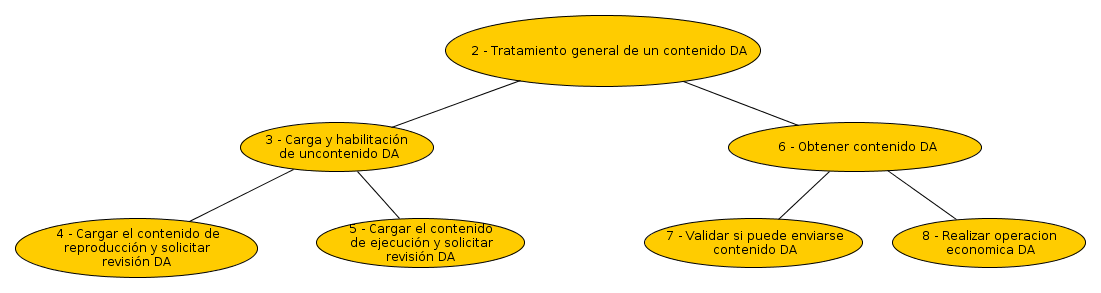
\includegraphics[scale=0.37]{Diagramas/00-DiagramaDeDiagramas.png}
	\end{center}

\subsubsection{Tratamiento general de un contenido}

	\begin{center}
		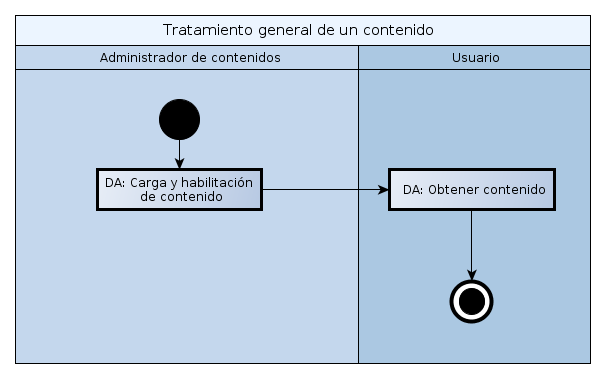
\includegraphics[scale=0.56]{Diagramas/02-TratamientoGeneralDeUnContenidoDA.png}
	\end{center}

\newpage

\subsubsection{Carga y habilitaci\'on de contenido}

	\begin{center}
		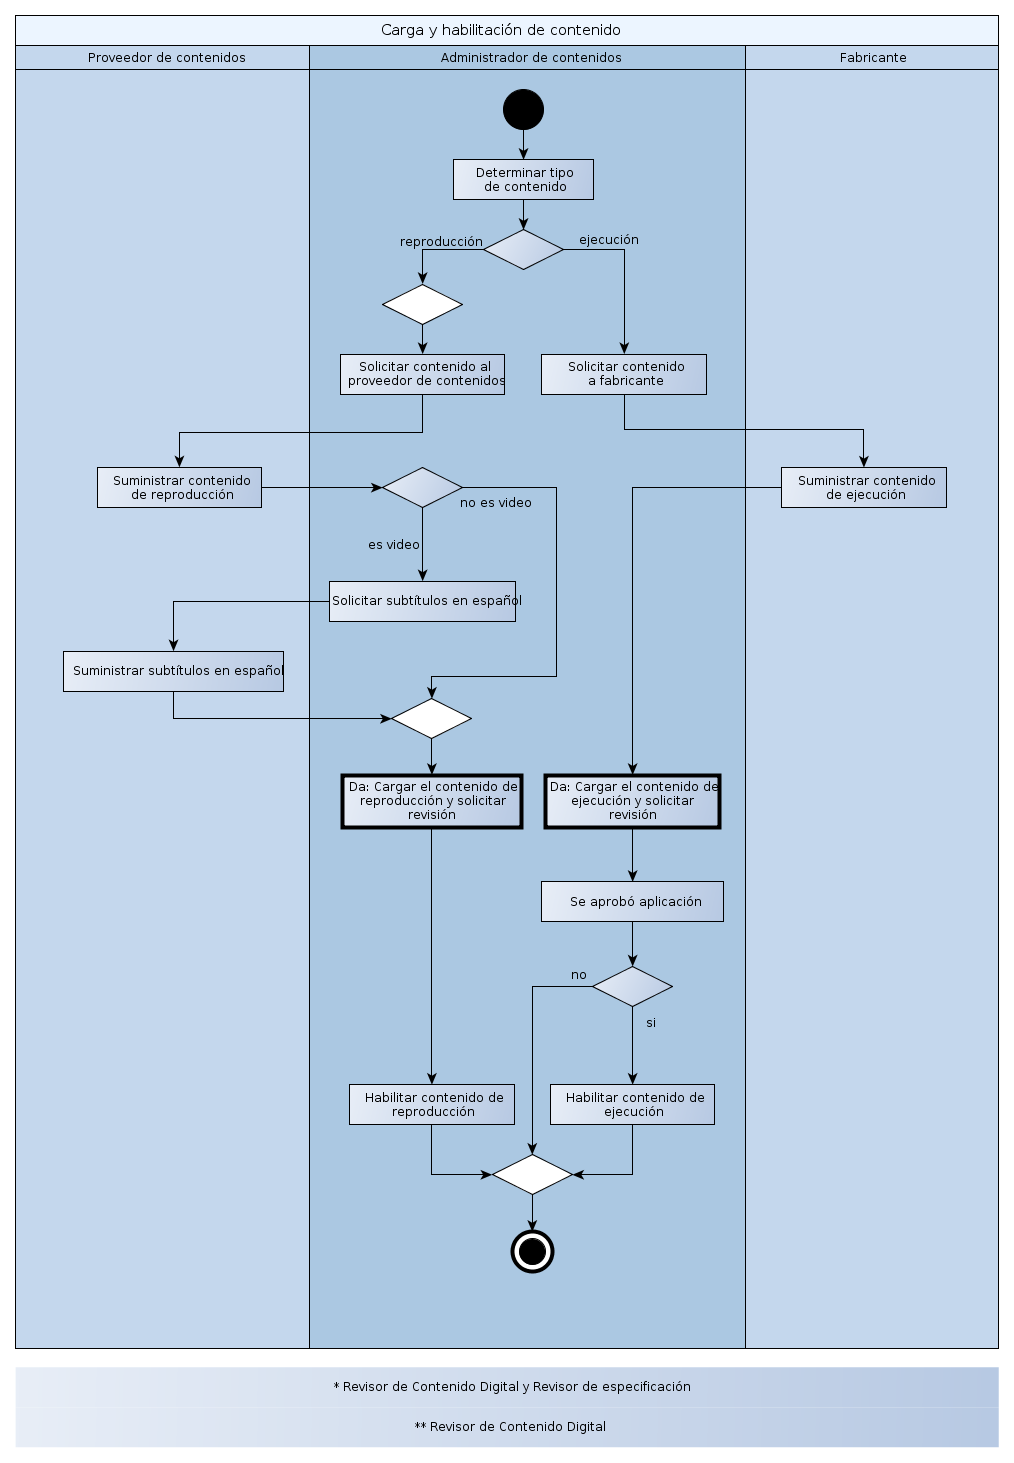
\includegraphics[scale=0.44]{Diagramas/03-CargaYHabilitacionDeContenidoDA.png}
	\end{center}
\newpage

\subsubsection{Cargar el contenido de reproducci\'on y solicitar revisi\'on}

	\begin{center}
		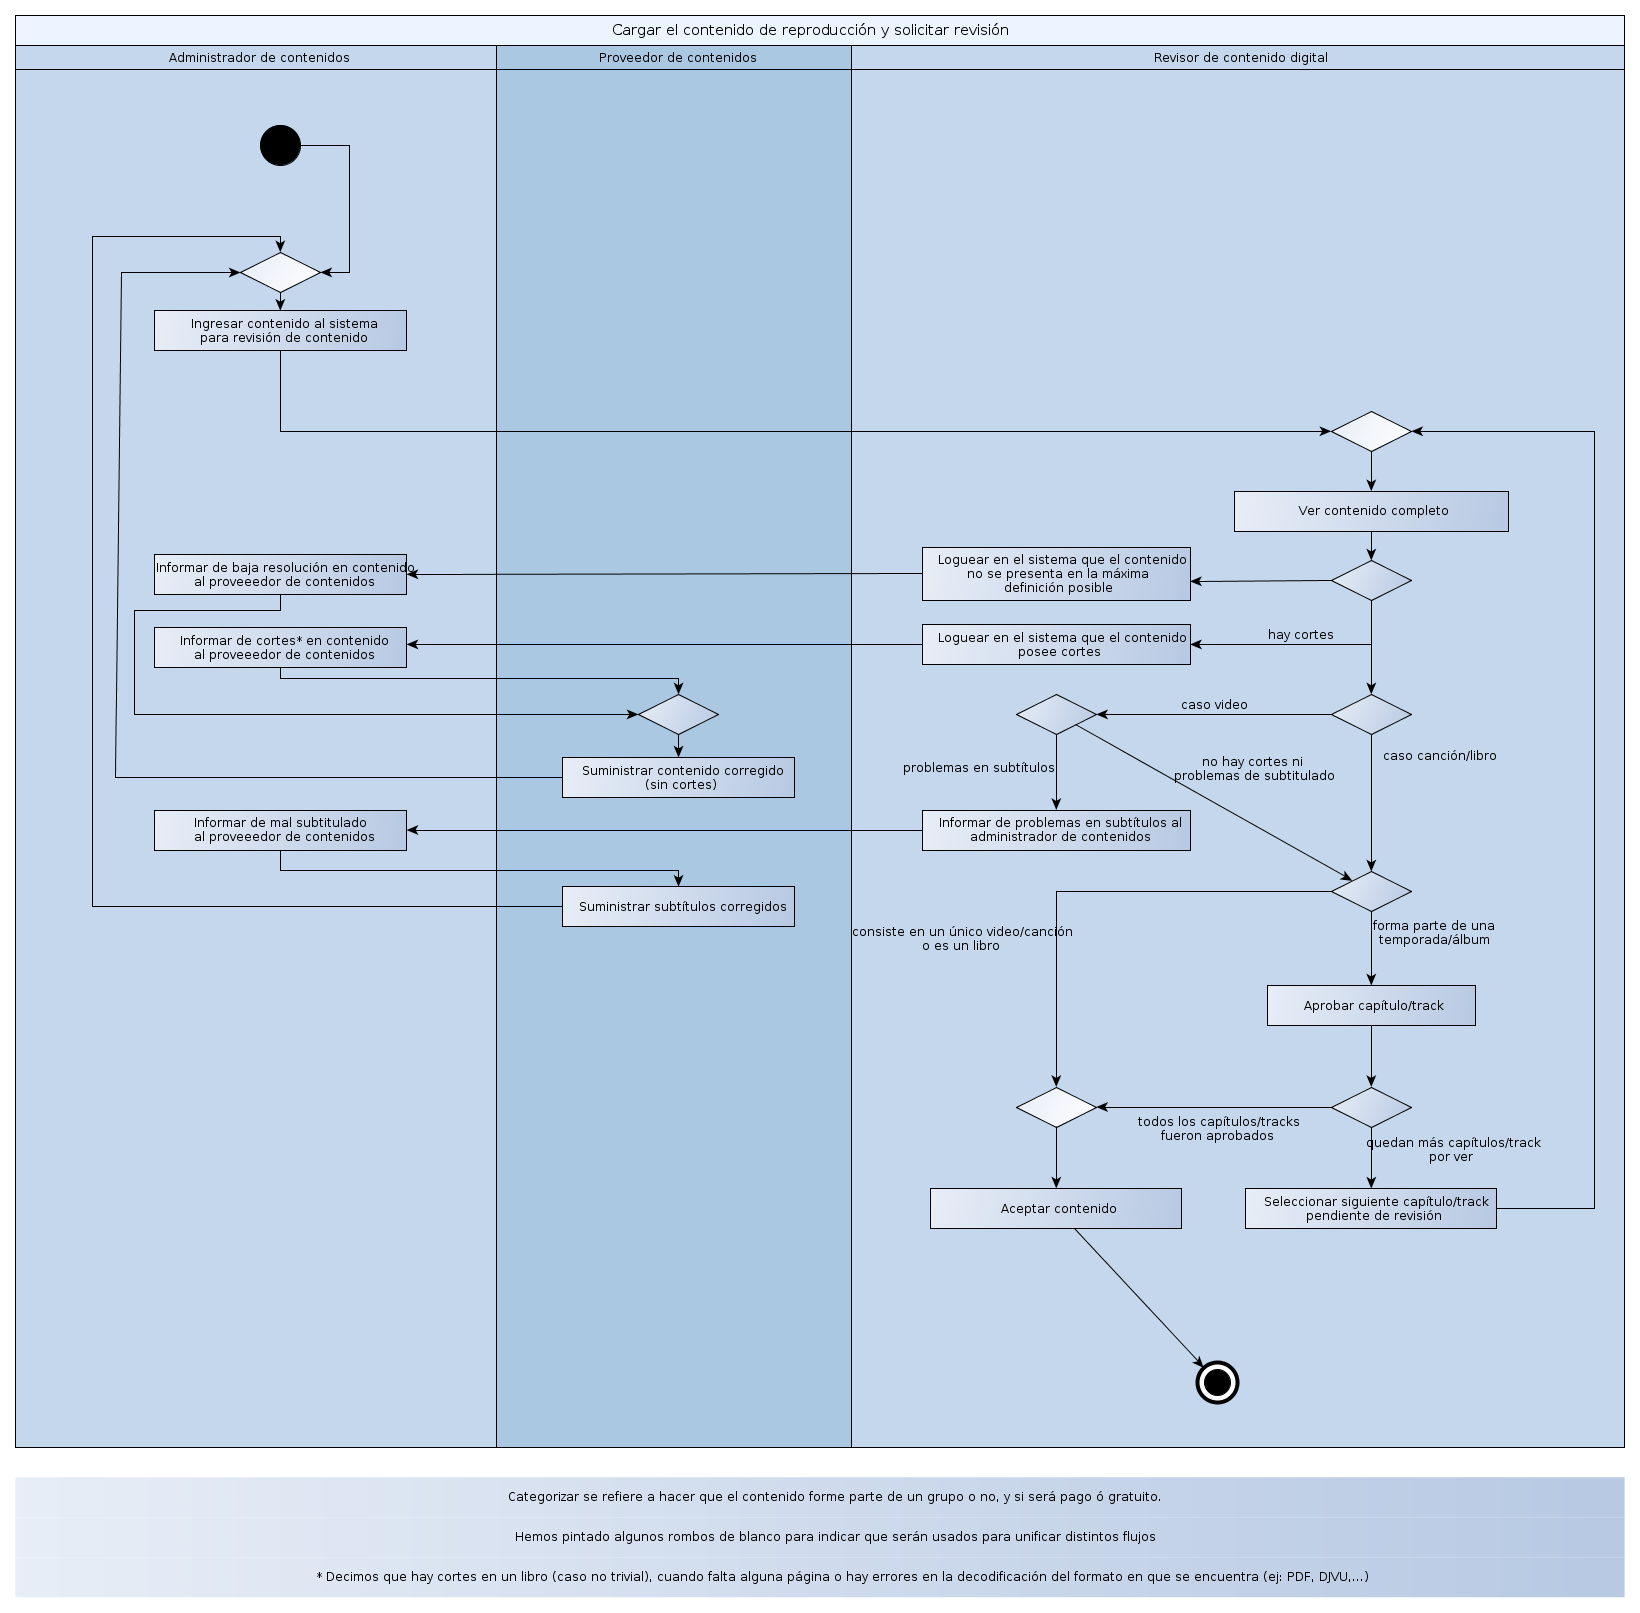
\includegraphics[scale=0.30]{Diagramas/04-CargarElContenidoDeReproduccionYSolicitarRevisionDA.png} 
	\end{center}

\newpage

\subsubsection{Cargar el contenido de ejecuci\'on y solicitar revisi\'on}

	\begin{center}
		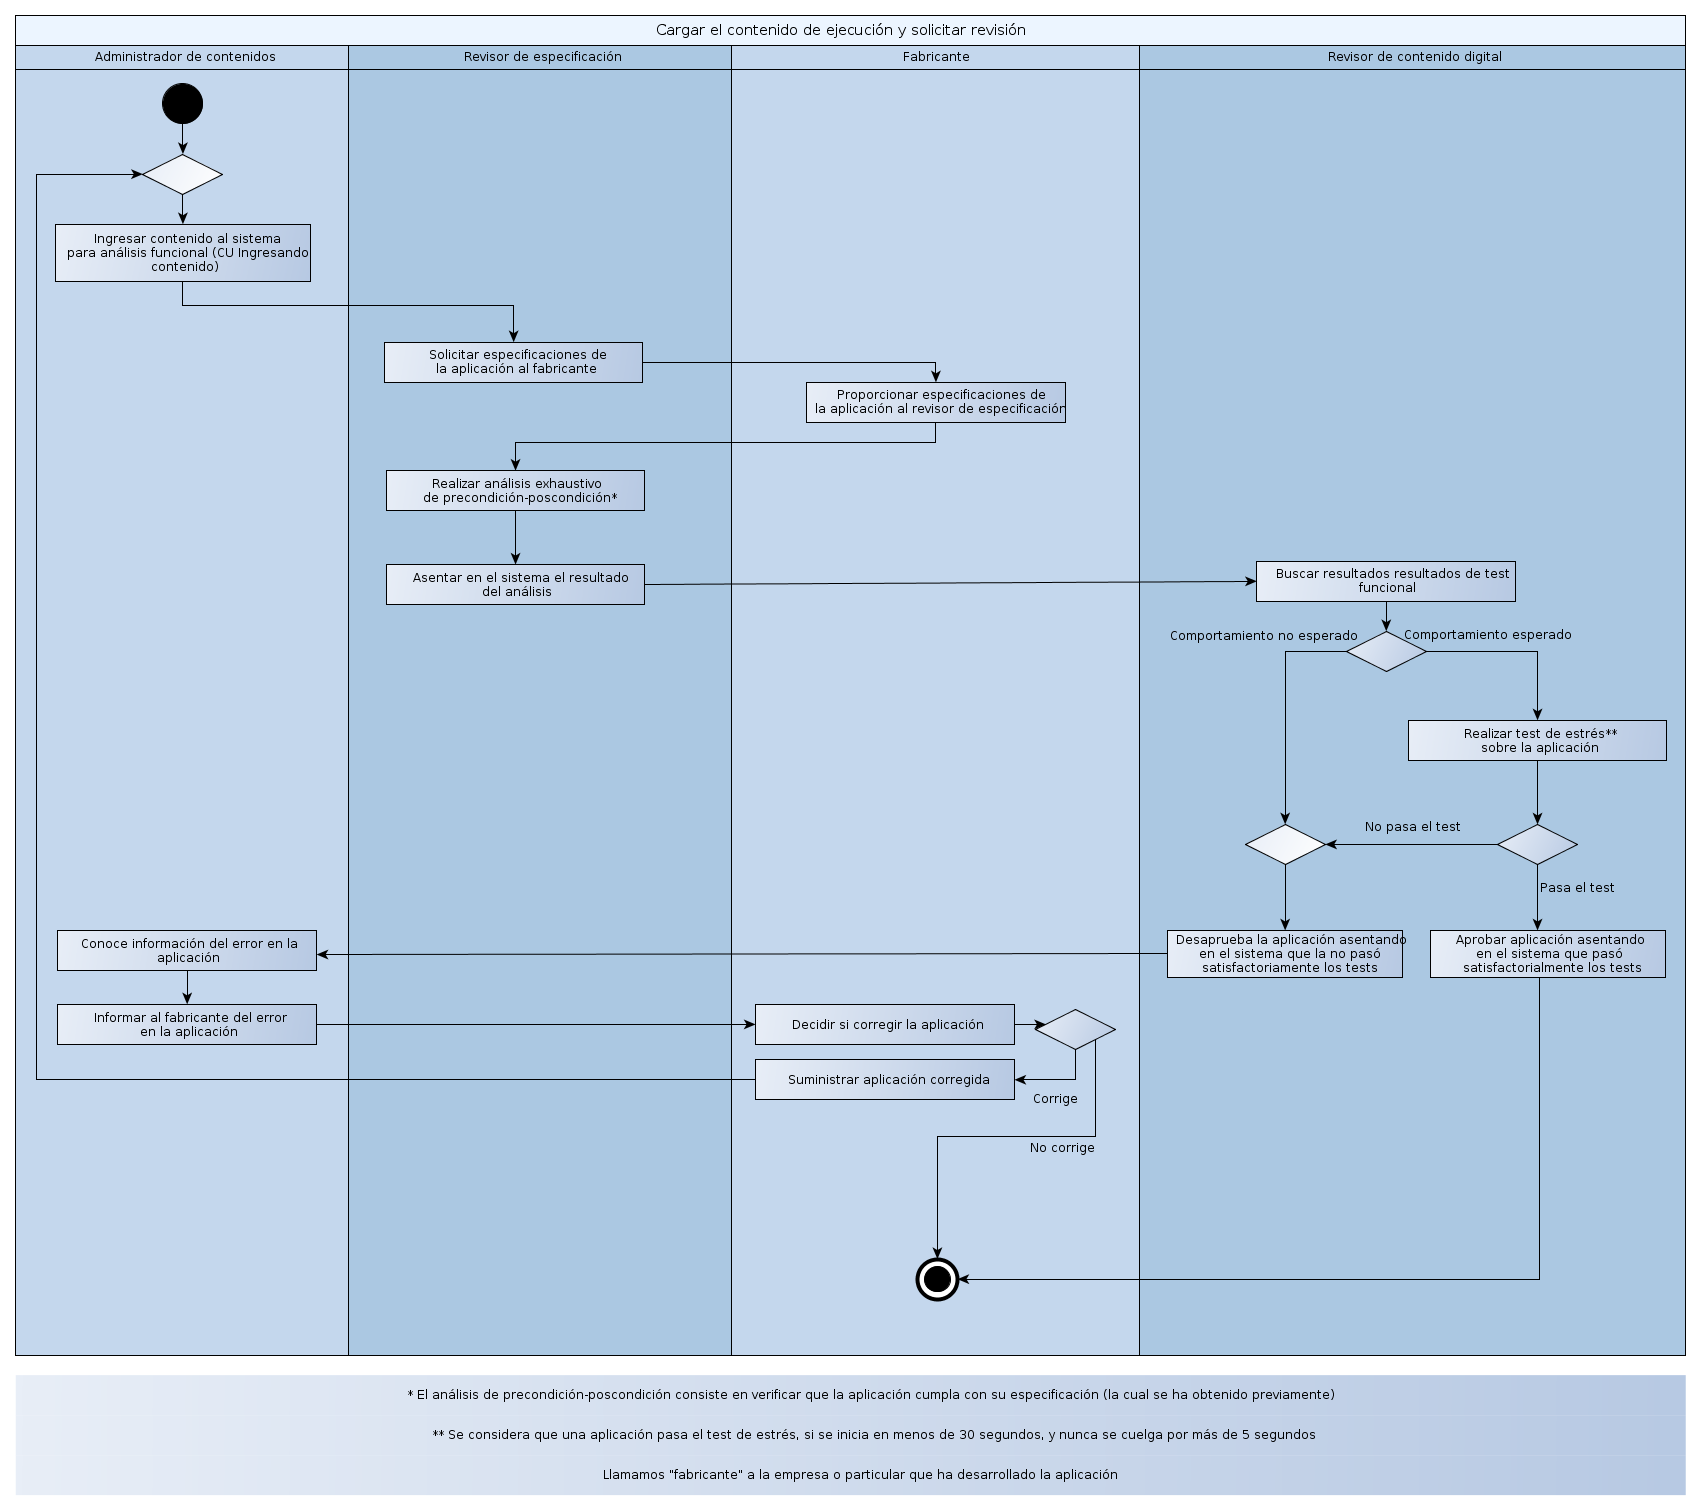
\includegraphics[scale=0.30]{Diagramas/05-CargarElContenidoDeEjecucionYSolicitarRevisionDA.png}
	\end{center}

\newpage

\subsubsection{Obtener contenido}

	\begin{center}
		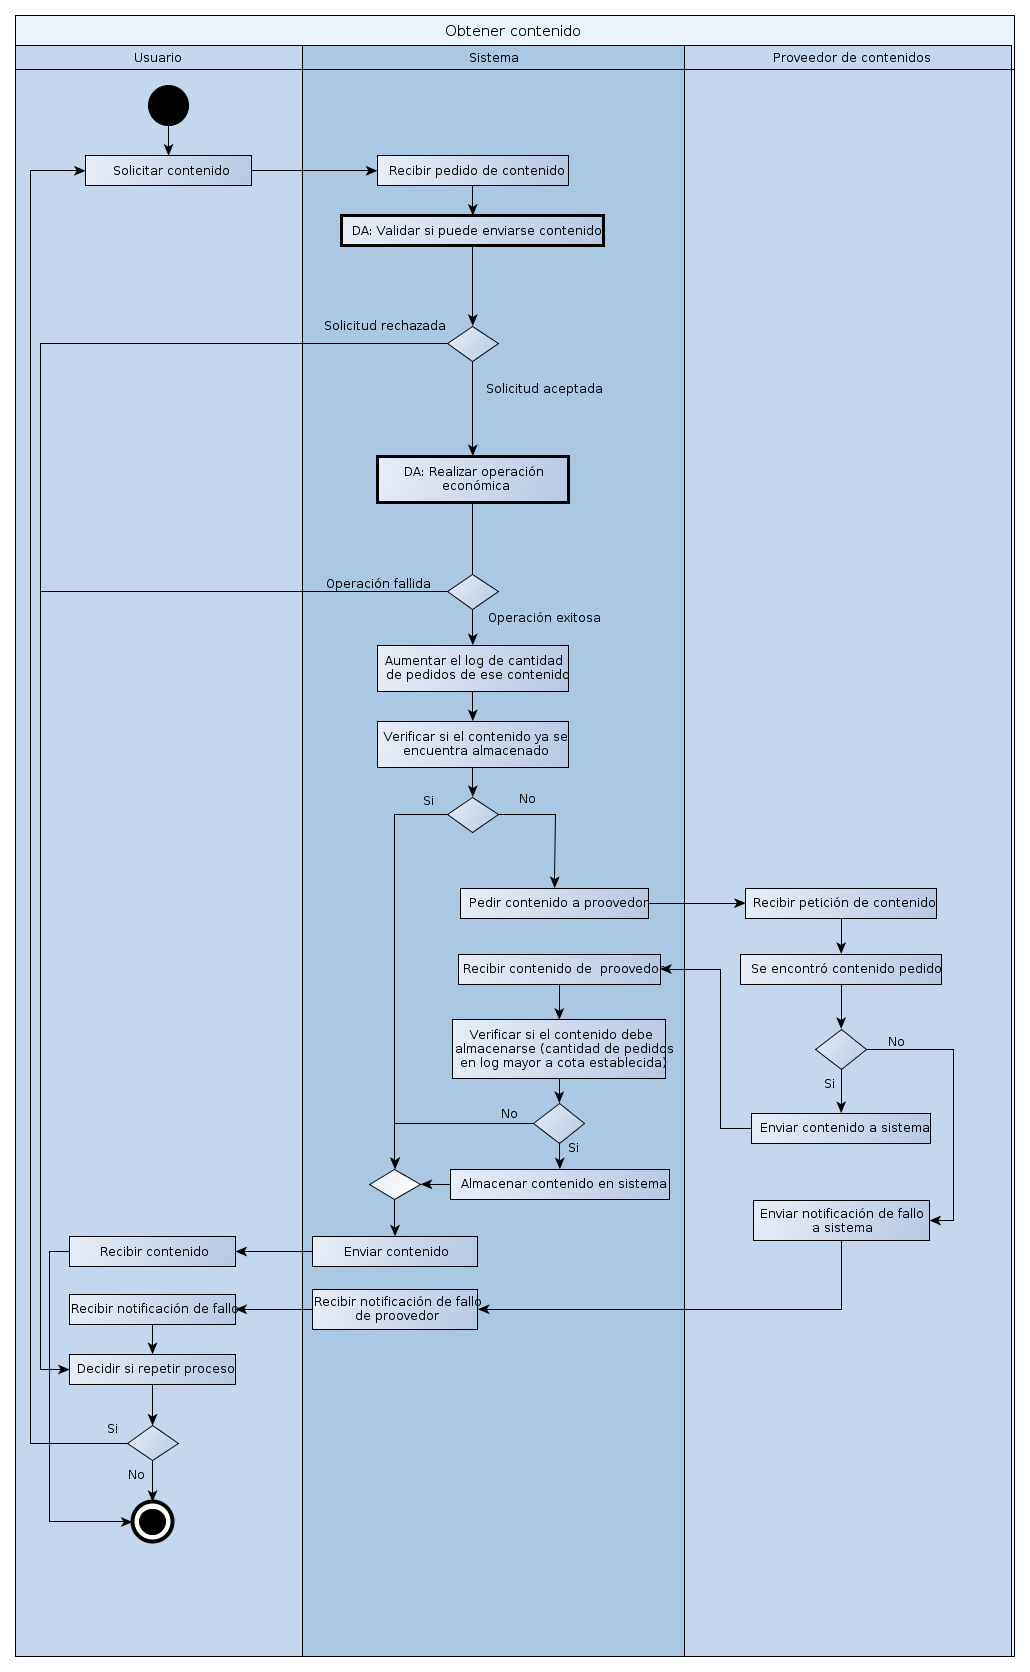
\includegraphics[scale=0.43]{Diagramas/06-ObtenerContenidoDA.png}
	\end{center}

\newpage

\subsubsection{Validar si puede enviarse contenido}

	\begin{center}
		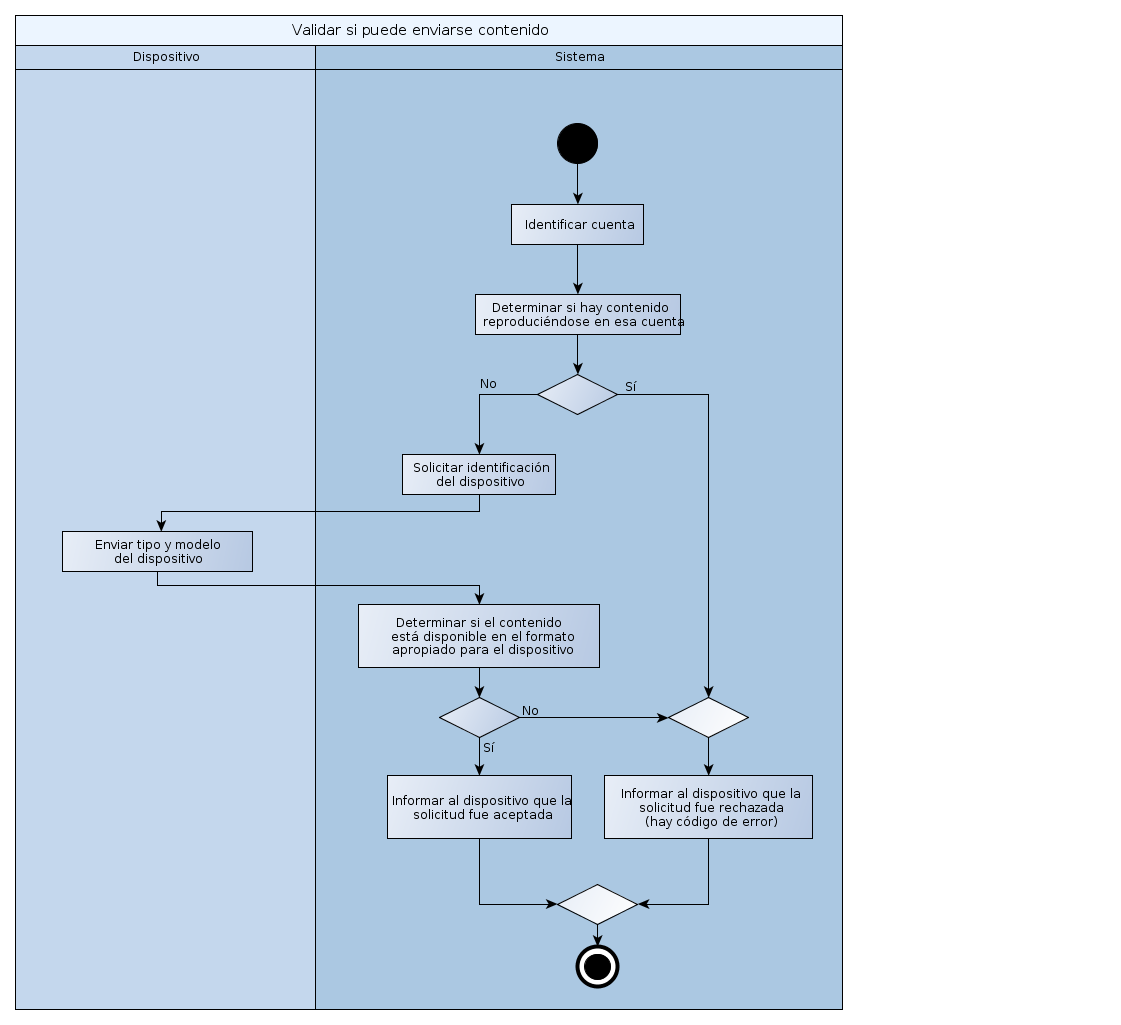
\includegraphics[scale=0.55]{Diagramas/07-ValidarSiPuedeEnviarseContenidoDA.png}
	\end{center}

\newpage

\subsubsection{Realizar operaci\'on econ\'omica}

	\begin{center}
		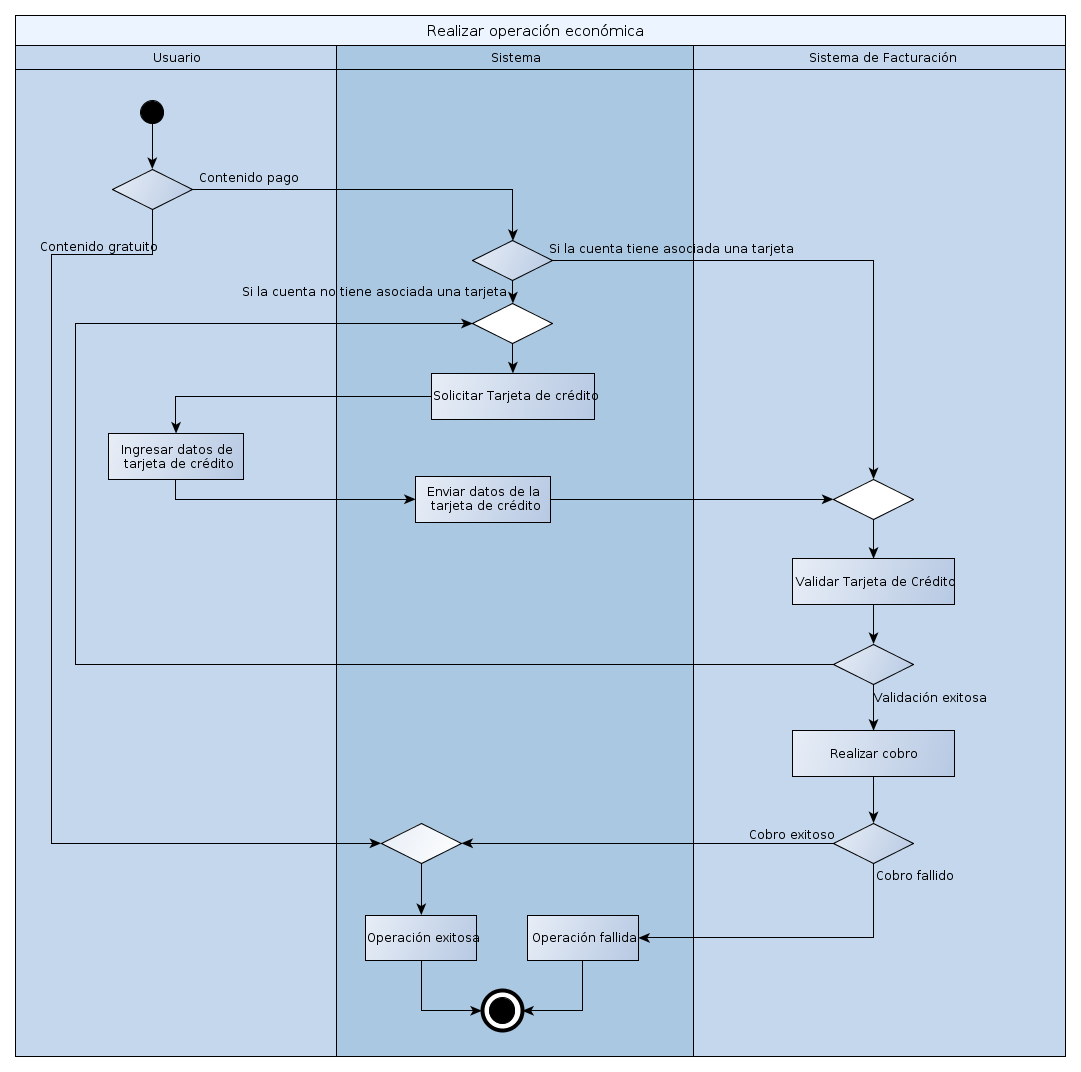
\includegraphics[scale=0.45]{Diagramas/08-RealizarOperacionEconomicaDA.png}
	\end{center}

\newpage

\subsection{Modelo Conceptual}

	\begin{center}
		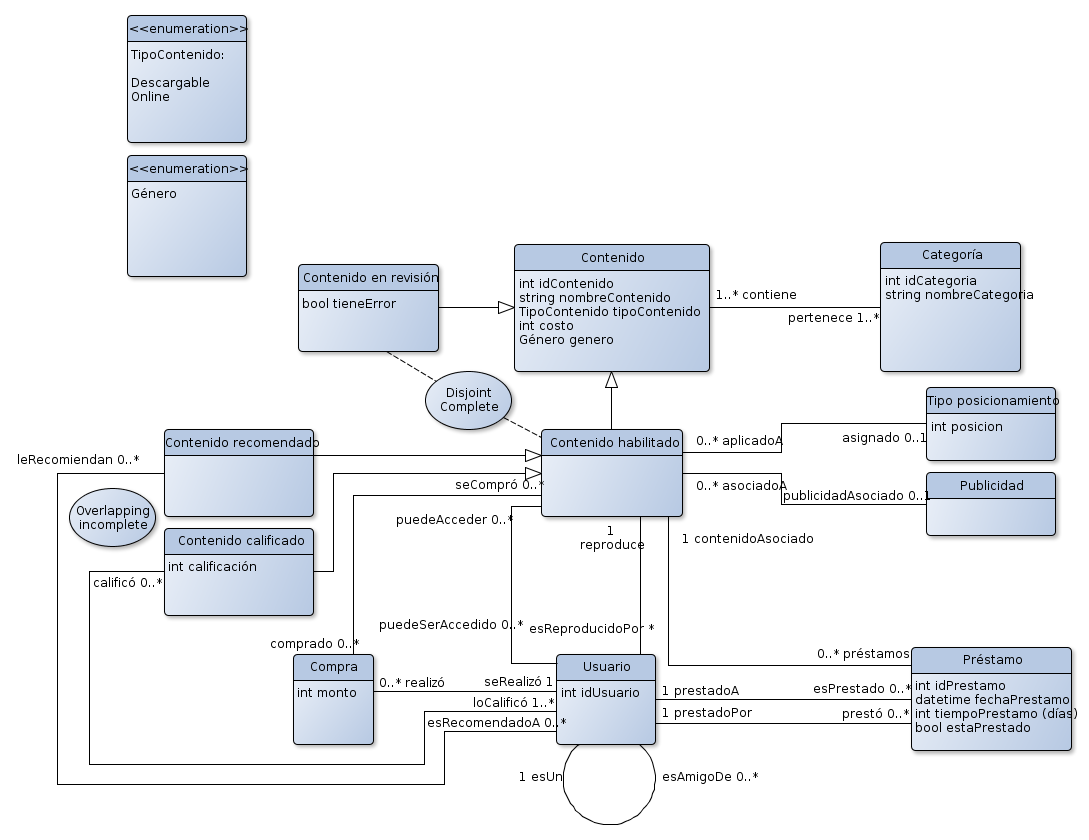
\includegraphics[scale=0.45]{Diagramas/09-ModeloConceptualMC.png}
	\end{center}

\subsubsection{Object Contraint Language (OCL)}
	Para complementar el \emph{Modelo Conceptual} agregaremos una serie de limitaciones que nos permiten modelar reglas para el sistema.
Este lenguaje nos permite especificar formalmente restricciones a las clases definidas.\\


\newpage
\begin{center} \line(1,0){450} \end{center}


\textbf{context Prestamos (prestamos valido)}\\
Los que se prestan son amigos (el id del usuario que recibe el pr\'estamo esta entre los ids de los amigos del usuario que presta\\
\noindent{\textbf{inv:} self.prestadoA.esAmigoDe $\rightarrow$ size() $>$ 0 $\wedge$}\\
self.prestadoA.esAmigoDe $\rightarrow$ includes( self.prestadoPor )\\
\begin{center} \line(1,0){450} \end{center}
\textbf{ Context: Pr\'estamo}\\
No se prestan contenidos de valor cero (contenidos gratis)\\
\noindent{\textbf{inv:} self.contenidoAsociado.monto $>$ 0}\\
\begin{center} \line(1,0){450} \end{center}
Si un usuario presta un contenido, debi\'o haberlo comprado \\
\noindent{\textbf{inv:} p.prestadoPor.realiz\'o$\rightarrow$ size()$>$0 and
p.prestadoPor.realiz\'o$\rightarrow$collect(seCompro)$\rightarrow$includes(p.ContenidoAsociado)}\\
\begin{center} \line(1,0){450} \end{center}
Los ids de los prestamos son diferentes\\
\noindent{\textbf{inv:} Prestamo.allIntances()$\rightarrow$forAll(i,j $\mid$ i $\ne$ j $\Rightarrow$ i.id $\ne$ j.id)}\\
\begin{center} \line(1,0){450} \end{center}
S\'olo se puede prestar contenido de tipo Online\\
\noindent{\textbf{inv:} self.contenidoAsociado.TipoContenido $=$ online}\\
\begin{center} \line(1,0){450} \end{center}
Ver q no haya coliciones de prestamos\\
\noindent{\textbf{inv:} Prestamo.allInstances()$\rightarrow$forAll( i , j $\mid$ i $\ne$j and i.prestadoPor $=$ j.prestadoPor $\Rightarrow$ ((i.contenidoAsociado $=$ j.contenidoAsociado)$\Rightarrow$ i.fechaPrestamo $>$ j.fechaPrestamo + j.tiempoPrestamo or i.fechaPrestamo+i.tiempoPrestamo $<$ j.fechaPrestamo or j.fechaPrestamo $>$ i.fechaPrestamo + i.tiempoPrestamo or j.fechaPrestamo + j.tiempoPrestamo $<$ i.fechaPrestamo ) }\\
\begin{center} \line(1,0){450} \end{center}
No puede pasar que si tengo un contenido prestado m\'as de una vez por la misma persona, que m\'as de un pr\'estamo figure como actualmente prestado, ni que hay un pr\'estamo con fecha de pr\'estamo posterior al del pr\'estamo que figure como actualmente prestado\\
   
\noindent{\textbf{inv:} Prestamo.allInstances()$\rightarrow$select(p $\mid$ p.estaPrestado)$\rightarrow$forAll(p$\mid$ not Prestamo.allInstances()$\rightarrow$Exists(p2 $\mid$ p2$\ne$p and (p.prestadoPor $=$ p2.prestadoPor and p.contenidoAsociado $=$ p2.contenidoAsociado and p2.estaPrestado or p.prestadoPor $=$ p2.prestadoPor and p.contenidoAsociado $=$ p2.contenidoAsociado and p2.fechaPrestamo $>$ p.fechaPrestamo)))}\\
\begin{center} \line(1,0){450} \end{center}
\textbf{Context Usuario}\\
Un usuario no puede ser amigo de si mismo\\
    \noindent{\textbf{inv:} self.esAmigoDe.size()$>$0 $\Rightarrow$ self.esAmigoDe()$\rightarrow$forAll( x $\mid$ x.usuarioId $\ne$ self.usuarioId)}\\
\begin{center} \line(1,0){450} \end{center}
El usuario tiene contenido recomendado sii calific\'o al menos un contenido\\
\emph{nota: not+xor equivale a si y s\'olo si}\\
\noindent{\textbf{inv:} not( self.califico.isEmpty() xor self.leRecomiendan.isEmpty() )}\\
\begin{center} \line(1,0){450} \end{center}
El usuario s\'olo calific\'o contenido que compr\'o (para todo contenido calificado, existe alguna compra hecha con ese contenido)\\
    \noindent{\textbf{inv:} self.califico$\rightarrow$forAll( u $\mid$ self.realizo$\rightarrow$exists( c $\mid$ c.seCompro.idContenido $=$ u.idContenido ))}\\
\begin{center} \line(1,0){450} \end{center}
Todos los contenidos tienen diferente id\\
\noindent{\textbf{inv:} Contenido.allIntances()$\rightarrow$forAll(c1,c2 $\mid$ c1 $\ne$ c2 $\Rightarrow$ c1.idContenido $\ne$ c2.idContenido)}\\
\begin{center} \line(1,0){450} \end{center}
La cantidad de contenidos recomendados a un usuario es igual a cero (si nunca calific\'o) o diez (cuando ya calific\'o)\\
\noindent{\textbf{inv:} self.leRecomiendan$\rightarrow$size() $=c$ 0 or self.leRecomiendan$\rightarrow$size()$=$ 10}\\
\begin{center} \line(1,0){450} \end{center}
La aparici\'on de cada g\'enero en el contenido recomendado a un usuario es proporcional a la suma de las calificaciones que el usuario le di\'o a contenido de ese g\'enero, sobre la suma de calificaciones totales.\\
No se recomienda contenido ya comprado ni contenido obtenido de pr\'estamos\\
\noindent{\textbf{inv:} self.leRecomiendan$\rightarrow$forall(c $\mid$ not c.comprado(isEmpty()) $\Rightarrow$ c.comprado$\rightarrow$forall(c2$\mid$ c2.seRealiz\'o.idUsuario $\ne$ self.seRealiz\'o.idUsuario)}\\
\begin{center} \line(1,0){450} \end{center}
Se puede reproducir s\'olo la reproduccion online\\
\noindent{\textbf{inv:} self.reproduce.size() $=$1 $\Rightarrow$ self.reproduce.TipoContenido $=$ Online}\\
\begin{center} \line(1,0){450} \end{center}
Se puede reproducir s\'olo lo que compro y no prest\'o, o pidi\'o prestado\\
\noindent{\textbf{inv:} self.Reproduce.size() $=$ 1 $\Rightarrow$ self.realizo$\rightarrow$collect(seCompr\'o)$\rightarrow$includes(self.Reproduce) and
self.Reproduce.pr\'estamos$\rightarrow$forall(p $\mid$ p.esPrestadoPor $=$ self $\Rightarrow$ not p.estaPrestado))) or
self.Reproduce.pr\'estamos$\rightarrow$exists(p2 $\mid$ p2.esPrestadoA $=$ self $\Rightarrow$p2.estaPrestado)))} \\
\begin{center} \line(1,0){450} \end{center}
No hay dos usuarios iguales. Todos los usuarios tienen diferente id\\
\noindent{\textbf{inv:} Usuario.allInstances()$\rightarrow$forAll(u1, u2 $\mid$ u1$\ne$u2 $\Rightarrow$ u1.idUsuario$\ne$u2.idUsuario)}\\
\begin{center} \line(1,0){450} \end{center}
\textbf{Context Contenido Calificado}\\
El contenido se califica de 0 a 10.\\
\noindent {\textbf{inv:} 0 $\leq$ self.calificacion and self.calificacion $\leq$ 10}\\
\begin{center} \line(1,0){450} \end{center}
\textbf{Context Compra}\\
El monto de la compra es igual al costo del contenido\\
\noindent {\textbf{inv:} self.monto $=$ self.seCompro.costo}\\
\begin{center} \line(1,0){450} \end{center}
\textbf{Context Publicidad}\\
La publicidad s\'olo se aplica a contenido de precio igual a cero (contenido gratuito)\\
\noindent{\textbf{inv:} self.asociadoA$\rightarrow$size() > 0 $\Rightarrow$ (self.asociadoA$\rightarrow$forall(c $\mid$ c.costo >0)) } \\
\begin{center} \line(1,0){450} \end{center}




\newpage

\section{Trazabilidad}

	Trazabilidad de los Objetivos del Tp1 con los diagramas antes mencionados.

A continuaci\'on se mostrar\'a la relaci\'on entre los distintos diagramas
title: Diagrama de Objetivos
subtitle: 0. Lograr enviar exitosamente el contenido:
Queremos definir de qu\'e forma el contenido se va a enviar. Para eso el contenido se va a poder descargar o ver de forma online en el sistema. Los casos de uso Solicitando contenido, Eligiendo contenido, Reproduciendo contenido online, Descargando contenido tratan la interacci\'on que va a existir entre el usuario y el sistema para lograr lo pedido.
Podemos ver adem\'as en el modelo conceptual cu\'al es la relaci\'on entre el contenido y el usuario. Los casos de uso y escenarios fijan que no puede haber m\'as de un contenido reproduciendo en simult\'aneo, siendo reafirmado por el modelo conceptual.
En el diagrama de actividad de Obtener contenido se puede ver el ciclo que cumple la solicitud hasta que esta se responde.
subtitle: 1.:Lograr proveer contenido contenido gratuito y pago bajo demanda para generar ingresos
En esta secci\'on se quiere definir la forma en la que se consigue el contenido y c\'omo se busca generar ingresos mediante un sistema de descarga bajo demanda.
    Los casos de uso asociados al administrador de contenido y al proveedor de contenido muestran c\'omo se comporta el sistema cuando se ingresa un nuevo contenido, junto con la forma de categorizarlo. Se observa c\'omo se cumplen los objetivos para obtener el contenido y lograr el almacenamiento eficiente. En el diagrama de Agentes 2.3.2 se puede observar como el administrador de contenido interact\'ua con el proveedor de contenido y el camino hasta habilitarlo al p\'ublico. Se complementa con los casos de uso en donde muestra la forma de categorizar el contenido, alterando sus par\'ametros.
    Por otro lado, se observa c\'omo es la interacci\'on del sistema con el sistema de facturaci\'on para lograr cobrar el contenido, publicidad y posicionamiento. los casos de uso asociados al sistema de facturaci\'on muestran este comportamiento. El diagrama de Agentes 2.3.7 muestra como se realiza la operaci\'on econ\'omica.
    En el diagrama 2.4 se puede observar como esta categorizado el contenido, que cuenta con un G\'enero y categor\'eas. Estas son las que se utilizan para filtrar cuando se quiere elegir el contenido a adquirir, y siendo el G\'enero el que se utiliza para determinar qu\'e contenido ser\'a recomendado por el sistema.
subtitle: 2. Lograr que sea personalizado
    Se hizo hincapi\'e en el sistema de pr\'estamo, as\'i como en la recomendaci\'on de contenido para que el sistema sea personalizado.
Se cre\'o el rol de amigo para detallar el sistema de pr\'estamo en los casos de uso. Con las restricciones de OCL, se valid\'o el funcionamiento de los pr\'estamos, sin agregarse la clase de Amigo, ya que es un Usuario. El usuario as\'i tiene una relaci\'on as\'i mismo que representa a los amigos de ese usuario/cuenta.
La recomendaci\'on de contenido viene de la mano de la calificaci\'on de contenido y la recomendaci\'on de contenido. En el diagrama, se plantea un algoritmo para la calificaci\'on de contenido que utiliza las calificaciones previas hechas por el usuario para definir qu\'e contenido mostrarle dependiendo del g\'enero del contenido. En el modelo conceptual vemos las restricciones que se aplican a la estructura de clases para que se realicen la recomendaci\'on de contenido por parte del sistema. Por ejemplo, no se recomienda contenido salvo que el usuario haya calificado al menos uno de ellos. Adem\'as, como es objeto de CentralMarket generar ingresos, se tom\'o como pol\'itica s\'olo recomendar contenido pago.
subtitle: 3 - Lograr proveer el contenido de forma transparente   
    En esta secci\'on se muestra todo el comportamiento del sistema para lograr que el contenido se pueda seguir reproduciendo desde el \'ultimo estado en que se lo dej\'o. Los casos de uso muestran el accionar del sistema cuando uno se autentica, y como el sistema toma las medidas necesarias para lograr la transparencia. En el diagrama de actividad 3.3.6 se puede observar como el sistema interacciona con el dispositivo para validar el traspaso (si es que hubo un cambio de dispositivo) y determina si es posible o no la carga del contenido.
subtitle: 4 - Lograr calidad de contenido.
    Se busca proveer los contenidos de mayor calidad, para eso CentralMarket cuenta con revisores de contenido digital y de especificaci\'on. Se quiere que todo contenido que est\'e disponible a los usuarios cuente con un est\'andar de calidad. En los casos de uso relacionados al Revisor de contenido digital y Revisor de especificaci\'on se denota de qu\'e forma se valida que se superen los test. Adem\'as el administrador de contenido una vez que los test se realizan decide dado su resultado habilitarlo o no. El flujo se ve en los diagramas de actividad de 03 - Carga y habilitaci\'on de contenido DA, 04 - Cargar el contenido de reproducci\'on y solicitar revisi\'on DA, 05 - Cargar el contenido de ejecuci\'on y solicitar revisi\'on DA.
En el modelo conceptual s\'olo se denot\'o que existe un tipo de contenido especial llamado \emph{Contenido en revisi\'on} sin m\'as detalle.

\newpage

\end{document}
